
% v03, AL, 07/29/19
% v04, MAP, 07/30/19



% ****** Start of file apssamp.tex ******
%
%   This file is part of the APS files in the REVTeX 4.1 distribution.
%   Version 4.1r of REVTeX, August 2010
%
%   Copyright (c) 2009, 2010 The American Physical Society.
%
%   See the REVTeX 4 README file for restrictions and more information.
%
% TeX'ing this file requires that you have AMS-LaTeX 2.0 installed
% as well as the rest of the prerequisites for REVTeX 4.1
%
% See the REVTeX 4 README file
% It also requires running BibTeX. The commands are as follows:
%
%  1)  latex apssamp.tex
%  2)  bibtex apssamp
%  3)  latex apssamp.tex
%  4)  latex apssamp.tex
%
\documentclass[%
 reprint,
%superscriptaddress,
%groupedaddress,
%unsortedaddress,
%runinaddress,
%frontmatterverbose, 
%preprint,
%showpacs,preprintnumbers,
%nofootinbib,
%nobibnotes,
%bibnotes,
 amsmath,amssymb,
 aps,
%pra,
%prb,
%rmp,
%prstab,
%prstper,
%floatfix,
]{revtex4-1}

\usepackage{graphicx}% Include figure files
\usepackage{dcolumn}% Align table columns on decimal point
\usepackage{bm}% bold math
\usepackage{xcolor}
%\usepackage{hyperref}% add hypertext capabilities
%\usepackage[mathlines]{lineno}% Enable numbering of text and display math
%\linenumbers\relax % Commence numbering lines

%\usepackage[showframe,%Uncomment any one of the following lines to test 
%%scale=0.7, marginratio={1:1, 2:3}, ignoreall,% default settings
%%text={7in,10in},centering,
%%margin=1.5in,
%%total={6.5in,8.75in}, top=1.2in, left=0.9in, includefoot,
%%height=10in,a5paper,hmargin={3cm,0.8in},
%]{geometry}

\begin{document}

\preprint{APS/123-QED}

%%%

%\title{Spatially Embedding Network Models via a Deterrence Function and Characterizing Strengths of Embedding on Topology}

\title{Spatial Strength Centrality and the Effect of Spatial Embeddings on Network Architecture}

\author{Andrew Liu}
% \email{liuandrew@ucla.edu}
\affiliation{%
Department, of Mathematics, University of California, Los Angeles, 90095, USA
}%

\author{Mason A. Porter}
\affiliation{
Department, of Mathematics, University of California, Los Angeles, 90095, USA
}%

\date{\today}% It is always \today, today,
             %  but any date may be explicitly specified

\begin{abstract}
For many networks, it is useful to think of their nodes as being embedded in a latent space, and such embeddings can affect the probability of whether nodes are adjacent to each other. In this paper, we extend existing models of synthetic networks to spatial network models by incorporating deterrence functions. We start by extending an existing geographical fitness model by employing normally-distributed fitnesses, and we then develop spatial versions of preferential attachment and configuration models. We define a notion of ``spatial strength centrality'' to help characterize how strongly a spatial embedding affects network structure, and we examine spatial strength centrality on a variety of real and synthetic networks.

\end{abstract}

%\pacs{Valid PACS appear here}% PACS, the Physics and Astronomy
                             % Classification Scheme.
%\keywords{Suggested keywords}%Use showkeys class option if keyword
                              %display desired
\maketitle

%\tableofcontents

%%%%%%

{\bf map: various things to do:
\begin{enumerate}
\item{[MAP's note to self on some papers to cite:] I would like to cite a paper by Eleni Katifori, if possible (it seems that some of her stuff is relevant); I also want to cite one of Geoff Boeing's papers at some point [7/30/19: I'll now do this next time, as I am seeing sufficient imprecision and confusion in parts of the paper that those parts will need clarification, so I may as well add these final citations in the next round instead]; I also want to cite our paper Berthier et al (PNAS 2019), as we consider spatial ideas rather explicitly therein (including trying to separate geometry and topology); citing our about-to-go-live article Nauer et al. probably also makes sense}
%\item{go through all bold comments before returning to Andy (maybe I will be able to do them all on my own?)}
%\item{please make changes to text in a new color so that I can just go through the changed parts of the paper when I see this again}
%\item{need to go back to the title of the paper (after I read through the whole paper)}
%\item{need to go back to the abstract of the paper}
% \item{maybe cite that paper Dani Bassett wrote with Florian Klimm and Peter Mucha, and maybe some other spatial neural ones from Dani? (what other spatial papers should we cite? Marta Sarzynska et al (see my website)? Paul Expert et al in ONAS?); there will need to be a paragraph to bring up some of these things; other papers that we could cite our my review article Papadopoulos et al. on granular and particulate networks, and also our recent paper Berthier et al (where we actually think about central geographical location a bit)}
%\item{Gastner--Newman model should be mentioned and cited in the intro to the paper (do you also do calculations on this later? considering that this interpolates between 2D and 3D, this seems like an important example for us to consider)}
%\item{(MAP note to self): there is a bike-share paper that we're finishing up that I may want to cite; I expect that one will be finished before this one, so for now I'll leave this note here, and I will take a look at it again when a new draft comes back to me later}
% \item{is there any other related work that we should bring up in the introduction? (we appear to be rather short on references to related work)}
% \item{I cleaned up the bibliography; make sure to cite the published versions of papers that are already published (rather than their arxiv versions), and also make sure to include all necessary coordinates (e.g., article number, which is the modern form of pages) in the .bib entries}
\end{enumerate}
}

%%%%%%


\section{Introduction} \label{sec:introduction}

Many networks have important spatial features, and it is often useful to think of the nodes of such spatial networks as being embedded in either a physical or a latent space \cite{barthelemy,newman2018}. In nature, such a latent space can be literal, like the physical distance between different parts of a city, or they can be more abstract. In social networks, for example, one can construe the nodes that represent individuals as having a distance between them that represents physical distance; a distance between them that arises from demographic characteristics, interests, behaviors, or other features; or a combination of such distances \cite{social}. In food webs, nodes that represent individuals can be embedded in a latent 
%one-dimensional 
space that represents various
 %size and other 
 features and affects their likelihood of interacting with each other. 
For instance, in a niche model, species are placed on a line, with a position that represents their mass and directed edges between nodes to represent who eats whom \cite{foodwebs}.
 
Physical networks, such as transportation networks and other networks within and between cities, possess a natural spatial embedding based on their physical location in the world. Whether networks are embedded in an explicit or latent space (or both), the distances between nodes can strongly influence whether they are adjacent to each other in a network \cite{spatial1, air-traffic, routelengthstatistic}. Intuitively, nodes that are farther apart from each other have fewer opportunities to interact (or their interaction has a greater associated cost), so we expect that there is a concomitant lower probability to observe edges between them. For example, people in a social network may be unlikely to interact if they share little in common \cite{socialdistance}, and animals in a food web may not hunt others that are too large or small in comparison to them \cite{foodwebs}. 

It is sensible that spatial characteristics should influence network structure, but it is much more difficult to make these ideas precise \cite{barthelemy}. For example, how exactly does a spatial embedding influence the architecture --- both topology and edge weights --- of a given network? For simplicity, most studies of networks have ignored spatial embeddings, but new models that incorporate spatial considerations are being developed with increasing frequency \cite{barthelemy}. 

Network models that incorporate space can improve measures of importance (i.e., centrality) of networks that are constructed from empirical data \cite{spatial1, air-traffic}. Additionally, spatially relevant features have been examined in brain networks \cite{braingrowth1, braingrowth2}, fungal networks \cite{fungal_data}, road networks {\color{red}\cite{road_data, spatial1, barbosa, boeing2018multi}}, air-traffic networks \cite{air-traffic}, gas-pipeline networks \cite{spatialefficiency}, and other applications. Incorporating spatial features can improve the modeling of empirical data \cite{barthelemy}, and it is therefore important to further extend ideas from network analysis into the realm of spatial networks.

Examples of spatial models include spatially-embedded random networks \cite{penrose-rgg, geographical_threshold} and networks that grow in time (e.g., through preferential attachment) \cite{mean_field_evolving_spatial, SPA1, spatial1}. Such models can provide reference models with which to compare empirical networks; and ideas from spatial networks have also led to spatial null models for community detection \cite{community1, community2}. %Additionally, s
Some spatial network models produce networks with multiple properties that are reminiscent of empirical networks (such as simultaneously having large values of clustering coefficients and heavy-tailed degree distributions \cite{geometric_preferential_attachment, geographical_threshold2}). Spatial network models have also been helpful for studying models of biological growth, such as osteocyte-network formation \cite{mean_field_evolving_spatial} {\color{red}or leaf venation networks \cite{leaf_optimization}.}

{\bf map: I wonder if the sentence above would be a good place to cite one of Eleni Katefori's papers}

{\bf map: in terms of urban structures (cities), I think we should cite Geoff Boeing at some point too}

{\bf andy: I wasn't entirely sure if these were the most appropriate papers that you had in mind. Please double check if these are okay!}


In the present paper, we explore a general approach for extending non-spatial network models to spatial versions by introducing a deterrence function \cite{community2}. This deterrence function $h(r)$, where $r$ represents the distance in either latent or physical space, modifies the probability that nodes are adjacent to each other as a function of the distance between them. 
{\color{red}We start by examining a modification of a geographical fitness (GF) model \cite{yusuke} that is a latent-space (``hidden variable'') model. Other works examining this GF model \cite{geographical_threshold, geographical_threshold2} have used exponential and power-law fitness functions, but we use one that is normally distributed. 
We then explore a spatial extension for the Barb\'abasi--Albert (BA) model, where this deterrence function modifies attachment probability for new edges (previous papers examine this \cite{SPA1, SPA2, SPA3}, but we incorporate the deterrence function slightly differently). Finally we apply this deterrence function for a configuration model \cite{fosdick} to create a spatial configuration model.
We compute some characteristics on these new spatial network models to understand how this deterrence function affects network topology. }
We also define a new spatial notion of centrality, which we call ``spatial strength centrality'' that helps us measure how strongly a spatial embedding affects the topological structure of a network. We examine how spatial strength centrality behaves on our new synthetic models, and we compute it for a variety of empirical spatial networks.

Our paper proceeds as follows. In Section \ref{sec:fitness_model}, we discuss GF models and explore the properties of these networks when using normally distributed fitnesses. {\color{red}We modify a spatial preferential attachment (SPA) model in Section \ref{sec:ba-model} and explore its properties, and develop a new spatial configuration model in Section \ref{sec:configuration_model}.} In Section \ref{sec:spatial_strength}, we define our notion of spatial strength centrality and apply it to several empirical and synthetic networks, including the models that we explored in previous sections. We conclude in Section \ref{sec:discussion}.



%%%%



\section{Geographical Fitness Model} \label{sec:fitness_model}

\subsection{Prior research}

The (non-geographical) fitness network model is a class of networks that assigns fitness values to the $n$ nodes of a network \cite{yusuke}. Such models are sometimes also called ``threshold models'' \cite{geographical_threshold}, although one needs to be careful not to confuse them with other similarly-named models \cite{newman2018}. One determines the intrinsic fitnesses of the nodes from a density function $f(w)$. In the original model \cite{caldarelli}, this intrinsic fitness characterizes the propensity of a node to gain edges. Such models have been used to generate small-world networks with power-law degree distributions \cite{geographical_threshold}.

One choice of fitness distribution is the exponential distribution
\begin{equation}\label{exponentialfitness}
    f(w) = \lambda e^{-\lambda w}\,, \quad w \geq 0\,.
\end{equation}
It gives the probability that a node has an intrinsic fitness value of $w$, where the parameter $\lambda \geq 0$ determines the shape of the distribution. An edge exists between nodes $v_i$ and $v_j$, with $i \neq j$, when 
\begin{equation} \label{chosen}
    g(i,j) = w_i + w_j \geq \theta \,,
\end{equation}
where $\theta$ is a ``threshold parameter'' that determines the fitness values that nodes need to be adjacent. With equation \eqref{chosen}, nodes that have a higher fitness value $w$ also have a larger degree. With either an exponential distribution or power-law distribution of fitness, one can show that the resulting degree distribution follows the power law $p(k) \sim k^{-2}$ as $k \rightarrow \infty$ \cite{caldarelli, threshold}.

One can also formulate geographical (or, more generally, spatial) versions of a fitness model, as illustrated in \cite{geographical_threshold, boguna, caldarelli}. In one extension, a network exists in a $d$-dimensional Euclidean space of finite size, such as in $[0, 1] \times [0, 1] \subset \mathbb{R}^2$ for $d = 2$. In addition to assigning node fitnesses using the distribution $f(w)$, one now also assigns a location in space to each node $v_i$. For example, perhaps one determines each of the node's $d$ coordinates uniformly at random in the space. One can then suppose that an edge exists between nodes $v_i$ and $v_j$, with $i \neq j$, when
\begin{equation}
    g(i, j, r) = (w_i + w_j)h(r) \geq \theta \,,
\end{equation}
where $r$ is the Euclidean distance between nodes $v_i$ and $v_j$ and the function $h(r)$ describes the influence of space on the connection probability of two nodes as a function of the distance between them. The function $h(r)$ is sometimes called a ``deterrence function'' \cite{barbosa}, and it has been used in many studies of spatial networks \cite{barthelemy}. A common choice for a deterrence function is the power-law form \cite{geographical_threshold}
\begin{equation}\label{distance_equation}
    h(r) = r^{-\beta}\,,
\end{equation}
for some value of a spatial decay parameter $\beta$. For certain values of $\beta$, it is possible to determine exact expressions for degree distributions and global clustering coefficients for the resulting fitness-network model \cite{geographical_threshold}, but most investigations with this deterrence function have focused on numerical computations. 


%%%%

\subsection{Normally-distributed fitnesses}

In previous treatments of (geographical and non-geographical) fitness network models, exponential and power-law distributions have been very common choices, including for the specific purpose of generating networks with power-law degree distributions \cite{geographical_threshold, geographical_threshold2, caldarelli, boguna}.

In the present study, we use a normal distribution for fitness, rather than an exponential or power-law distribution. We make this choice based on the intuition that entities (which are represented by nodes) have a variety of intrinsic factors that influence whether they interact with other nodes in a system, so this is a plausible choice in many situations \cite{frank}. 
We chose a standard normal distribution
\begin{equation}
        W {\raise.17ex\hbox{$\scriptstyle\mathtt{\sim}$}} N(0, 1)\,.
\end{equation}
We also modify the threshold function and write
\begin{equation}
    g(i, j, r) = |w_i - w_j| h(r) \geq \theta\,,
\end{equation}
such that nodes that differ widely in intrinsic fitness are more likely to interact with each other than those with similar intrinsic fitness. That is, we generate networks with disassortative mixing with respect to node fitness. Possibilities where this may be relevant may be hyperlinks from many low-fitness Web pages to high-fitness ones and predators in a food web hunting much weaker prey.
%For example, perhaps Web pages with less traffic link preferentially to ones with more traffic, or perhaps predators in a food web are more likely to hunt weaker prey than each other.

%%%%

\subsection{Network realizations and numerical computations}\label{sec:fitness_numerics}

For our numerical computations, we construct networks with $n = 500$ nodes that are embedded in $2$-dimensional (2D) space in a box $[0, 1] \times [0, 1]$ with periodic boundary conditions. The nodes have coordinates $(x_1, x_2)$, where we assign $x_1$ and $x_2$ independently with uniform probability on the interval $[0,1]$, and normally-distributed fitnesses with mean $\mu = 0$ and standard deviation $\sigma = 1$. 

For the threshold function \eqref{distance_equation}, we consider values $\beta \in \{ 0, 0.5, 1, 1.5, 2, 2.5, 3 \}$ for the decay parameter $\beta$, and we manually adjust $\theta$ such that the mean degree $\langle k \rangle = 20$. We obtain $\theta$ through a combination of trial-and-error and fitting through linear regression. We generate $30$ instances of these networks for each value of $\beta$.


\begin{figure*}
    \centering
    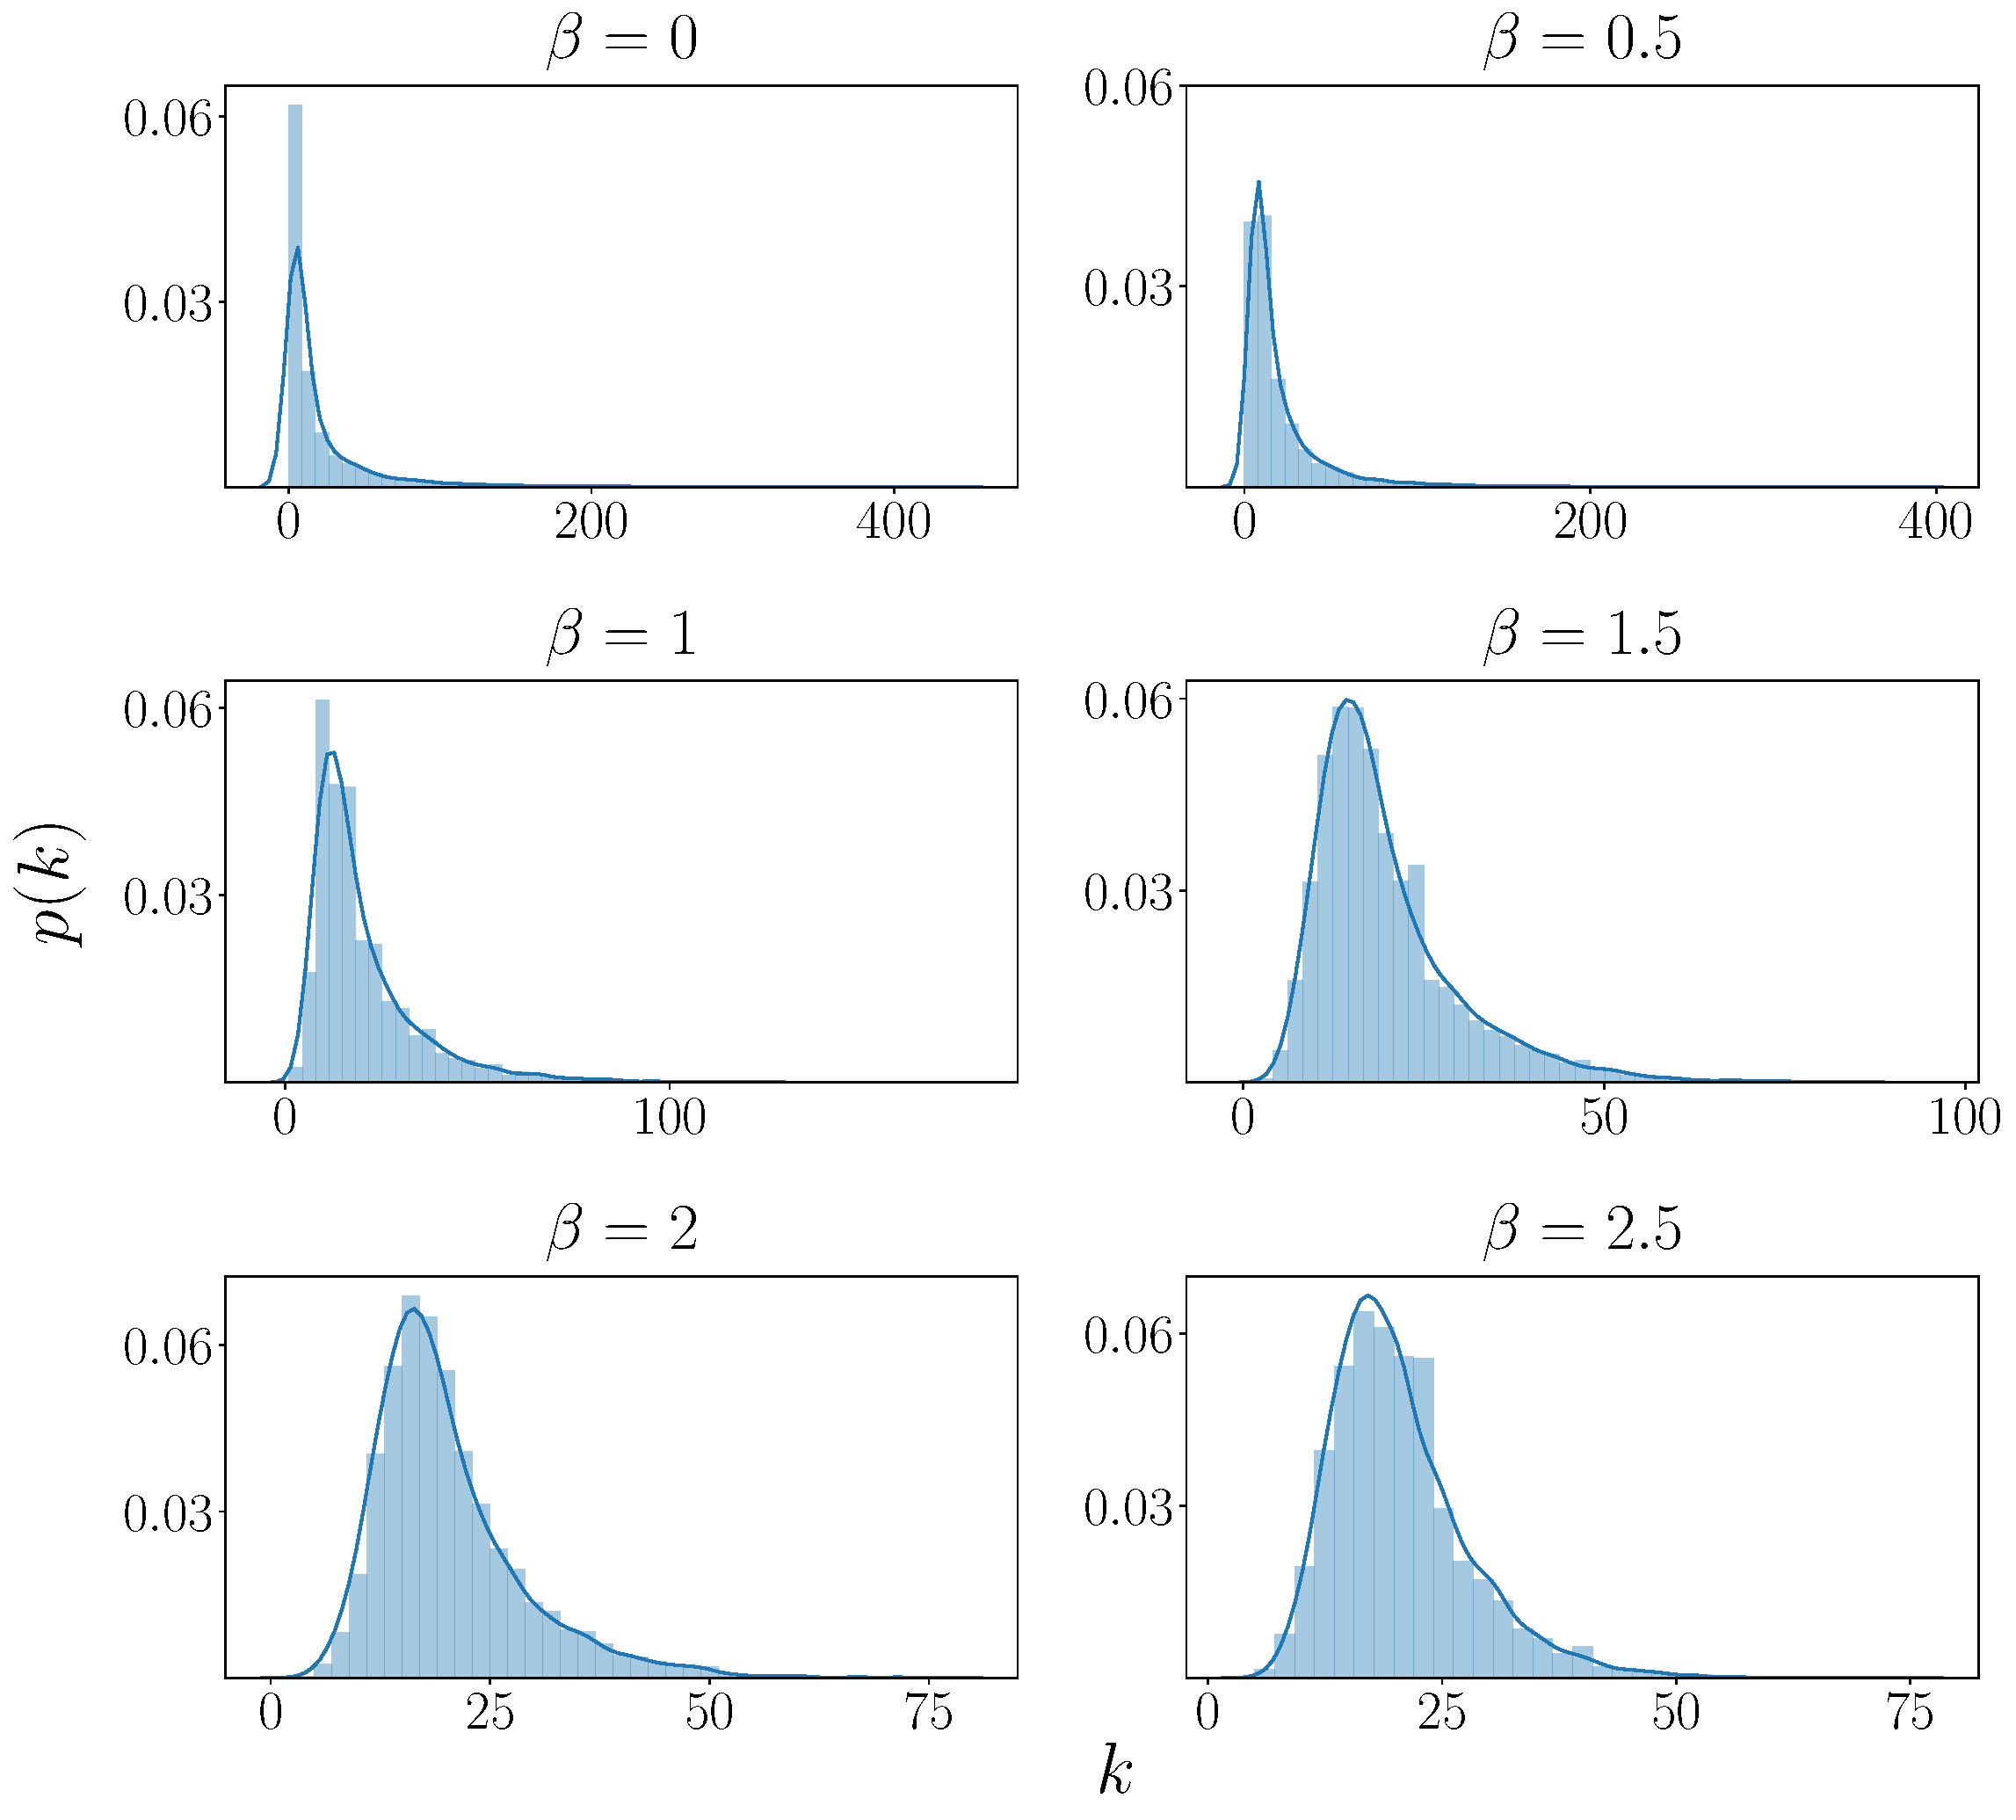
\includegraphics[width=0.7\linewidth]{geographical_degree_distribution3.pdf}
    \caption{Example degree distributions of geographical fitness networks with normally-distributed fitnesses and various values of the decay parameter $\beta$.
    }
\end{figure*}


When $\beta = 0$, we recover a non-geographical threshold model, where the distances between nodes do not play a role in the probability of nodes to be adjacent. In this regime, the distribution looks visually like it may satisfy a power law, although we do not test this idea.
%like it may be a power law, though further tests would be needed to confirm this. 
 For progressively larger values of $\beta$, distance plays a progressively stronger role, and nodes that are farther apart are less likely to be adjacent to each other.

We calculate a few well-known network characteristics \cite{newman2018} and find that they are affected by distance (as encoded in the value of $\beta$). The characteristics that we calculate are
\begin{enumerate}\label{characteristics_definitions}
    \item {\bf Mean local clustering coefficient.} The local clustering coefficient of a node with degree at least $2$ is $c_i = \frac{2T(v_i)}{k_i(k_i - 1)}$, where $T(v_i)$ is the number of unique triangles (i.e., $3$-cliques) to which node $v_i$ belongs and $k_i$ is the degree of node $v_i$. A node with degree $0$ or $1$ has a local clustering coefficient of $0$. {\color{red}The mean local clustering coefficient of a network is the mean value of $c_i$ over all nodes in the network (including nodes with degrees $0$ and $1$).} 
    \item {\bf Mean geodesic distance.} The mean geodesic distance is  $L = \frac{\sum_{i \neq j}d(v_i, v_j)}{n(n-1)}$, where $d(v_i, v_j)$ is the shortest-path distance (in terms of number of edges) between nodes $v_i$ and $v_j$.
    \item {\bf Mean edge length.} We take the length of an edge to be the Euclidean distance between its two incident nodes. The mean edge length of a network is the mean edge length over all edges in the network.
    \item {\bf Degree assortativity.} We calculate the degree assortativity of a network using {\color{red}the Pearson correlation coefficient} $r = \frac{\sum_{i,j}(A_{i,j}-k_i k_j/2m)k_i k_j}{\sum_{i,j}(k_i \delta_{i,j}-k_i k_j/2m)k_i k_j}$ \cite{newman2018}, the normalized covariance of degrees of the nodes of the network.
\end{enumerate}

%{\bf map: isn't $r$ above a Pearson correlation coefficient?}

Larger values of $\beta$ yield shorter mean edge lengths, larger mean geodesic lengths, and larger mean local clustering coefficients. In our plots in this section, we calculate the means of these characteristics in a network, and we then take the mean across 30 instantiations.
%over each each edge or node in the network, and then as a mean over all 30 instantiations. 
%The mean clustering coefficient of the network also becomes larger; this 
We note that this result for the mean local clustering coefficient is intuitively sensible, as nodes in small neighborhoods of nodes are more likely to be adjacent to each other for larger values of $\beta$ (i.e., as spatial effects become more prominent). 

To facilitate exposition, 
%throughout this paper, 
we use the term ``spatial effects'' to describe network topology and network characteristics being influenced by a spatial embedding, such that greater spatial effects signify more influence of a spatial embedding on a network.
%. The greater the spatial effects, the more a spatial embedding influences a network. 
With the deterrence function $h(r) = r^{-\beta}$, we expect spatial effects to increase as we increase $\beta$. The most obvious example of this phenomenon is with mean edge length, a network characteristic. With this model (and the subsequent ones in this paper), as we increase $\beta$, edges form more preferentially between spatially close nodes, so mean edge length decreases as we increase $\beta$. 


\begin{figure}
    \centering
    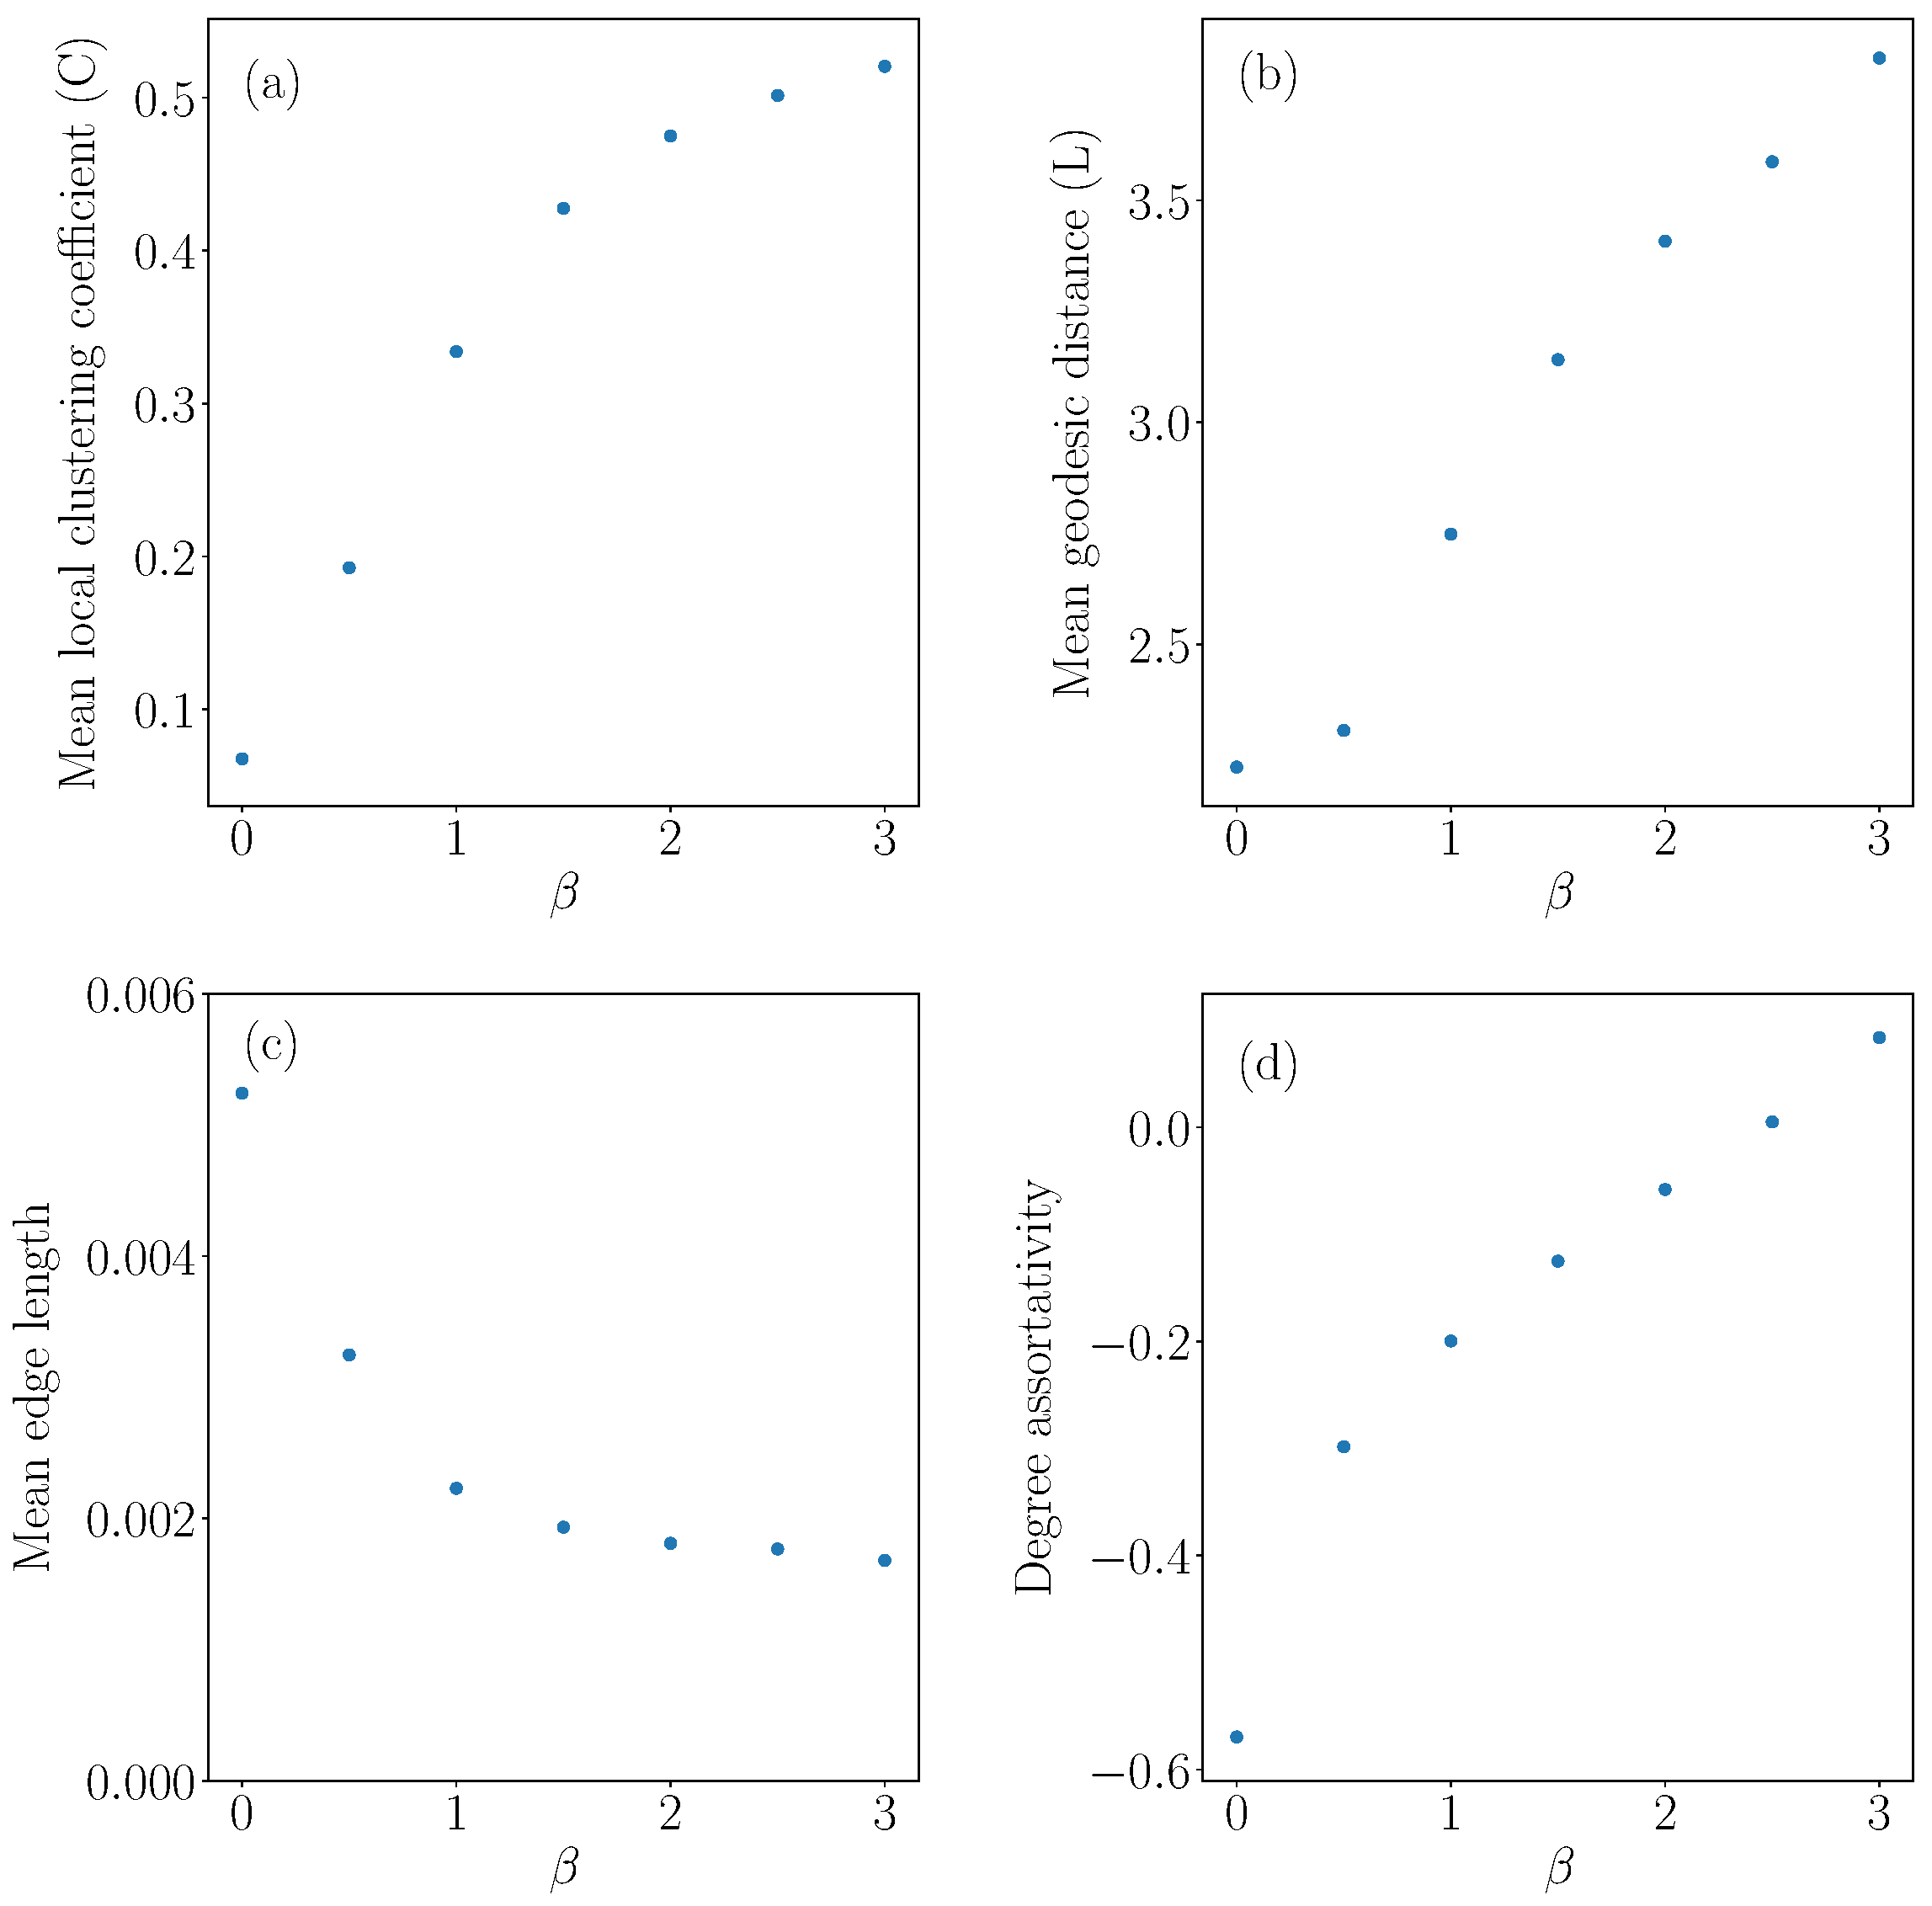
\includegraphics[width=1.0\linewidth]{geographical_network_metrics3.pdf}
    \caption{Characteristics of networks (with $n = 500$ nodes) from a geographical fitness models with normally-distributed fitness for different values of $\beta$ and $30$ instantiations of the model for each value of $\beta$. We show the (a) mean local clustering coefficient, (b) mean geodesic distance, (c) mean edge length, and (d) degree assortativity. In all cases, we first take means with respect to individual networks and then over the $30$ instantiations.
    }
    \label{fig:gf_metrics}
\end{figure}


Near $\beta = 0$, we observe a lower degree assortativity because of the heterogeneous mixing of nodes with different degrees. This is a consequence of how we formulated the model, as nodes with extreme fitness values (either positive or negative ones) yield larger values of $|w_i - w_j|$, so they are adjacent to all nodes with fitnesses that are sufficiently close to $0$. These nodes, whose fitnesses are in the center of the fitness distribution, are not likely to be adjacent to each other.

By contrast, for larger values of the decay parameter $\beta$ (e.g., for $\beta \geq 2$), the Euclidean distance between two nodes has more influence over the probability that they are adjacent. In this regime, it is no longer the case that nodes with extreme fitness are adjacent to all nodes in the network. 

If we let $\beta \rightarrow \infty$, we expect the distance between nodes to become the sole factor that determines whether nodes are adjacent. In our numerical computations, we hold $\langle k \rangle$ roughly constant at $20$, so we expect nodes to be adjacent to roughly $20$ of their nearest neighbors. In this respect, as $\beta \rightarrow \infty$, we expect the network to resemble a random geometric graph (RGG) \cite{penrose-rgg, rgg} with an appropriate value of the connection radius $r$. {\color{red}The RGG considered in this paper is a graph model that is given two parameters: the number of nodes $n$, and a connection radius $r_c$. Each node is added to a $[0, 1] \times [0, 1] \subset \mathbb{R}^2$ with its location assigned uniformly at random in the space. Pairs of nodes are adjacent to each other if their Euclidean distance is less than or equal to $r_c$ in the space. Thus adjacency in the network is determined completely by the position of its nodes. }

In an instantiation of the GF with $\beta=50$, an RGG (with periodic boundary conditions) with the same node positions and with $r \approx 11.3$ (thus having $\langle k \rangle \approx 20$) yields a network with $98\%$ of the same edges. {\color{red}The same experiment with $\beta=3$ yields $77\%$ of the same edges and with $\beta=1$ yields $52\%$ of the same edges (percentages are precise to 2 digits).} Random geometric graphs have positive degree assortativity \cite{rgg_correlations}, so as we increase $\beta$, we expect degree assortativity to increase to positive values that resemble those of this type of RGG. {\color{red}As shown in Fig \ref{fig:gf_metrics}, this indeed appears to be the case.}

%{\bf map (7/29/19): just a note (comment out after reading it): there is more than one type of RGG; you need to connect these comments to the specific type of RGG you have in mind, not to RGGs more generally; this is also why it's crucial that you include a precise definition of RGG above}


%%%%

\subsection{Closeness centrality}\label{close}

Normalized closeness centrality gives an idea of how ``close'' a node is to other nodes in a network, as determined by how many edges are between it and other nodes in the network \cite{newman2018}. The version of closeness centrality that we calculate is
\begin{equation}
    C(v_i) = \frac{n - 1}{\sum\limits_{i \neq j} l(v_i,v_j)}\,,
\end{equation}
where $l(v_i, v_j)$ is the geodesic distance between nodes $v_i$ and $v_j$.



\begin{figure}
    \centering
    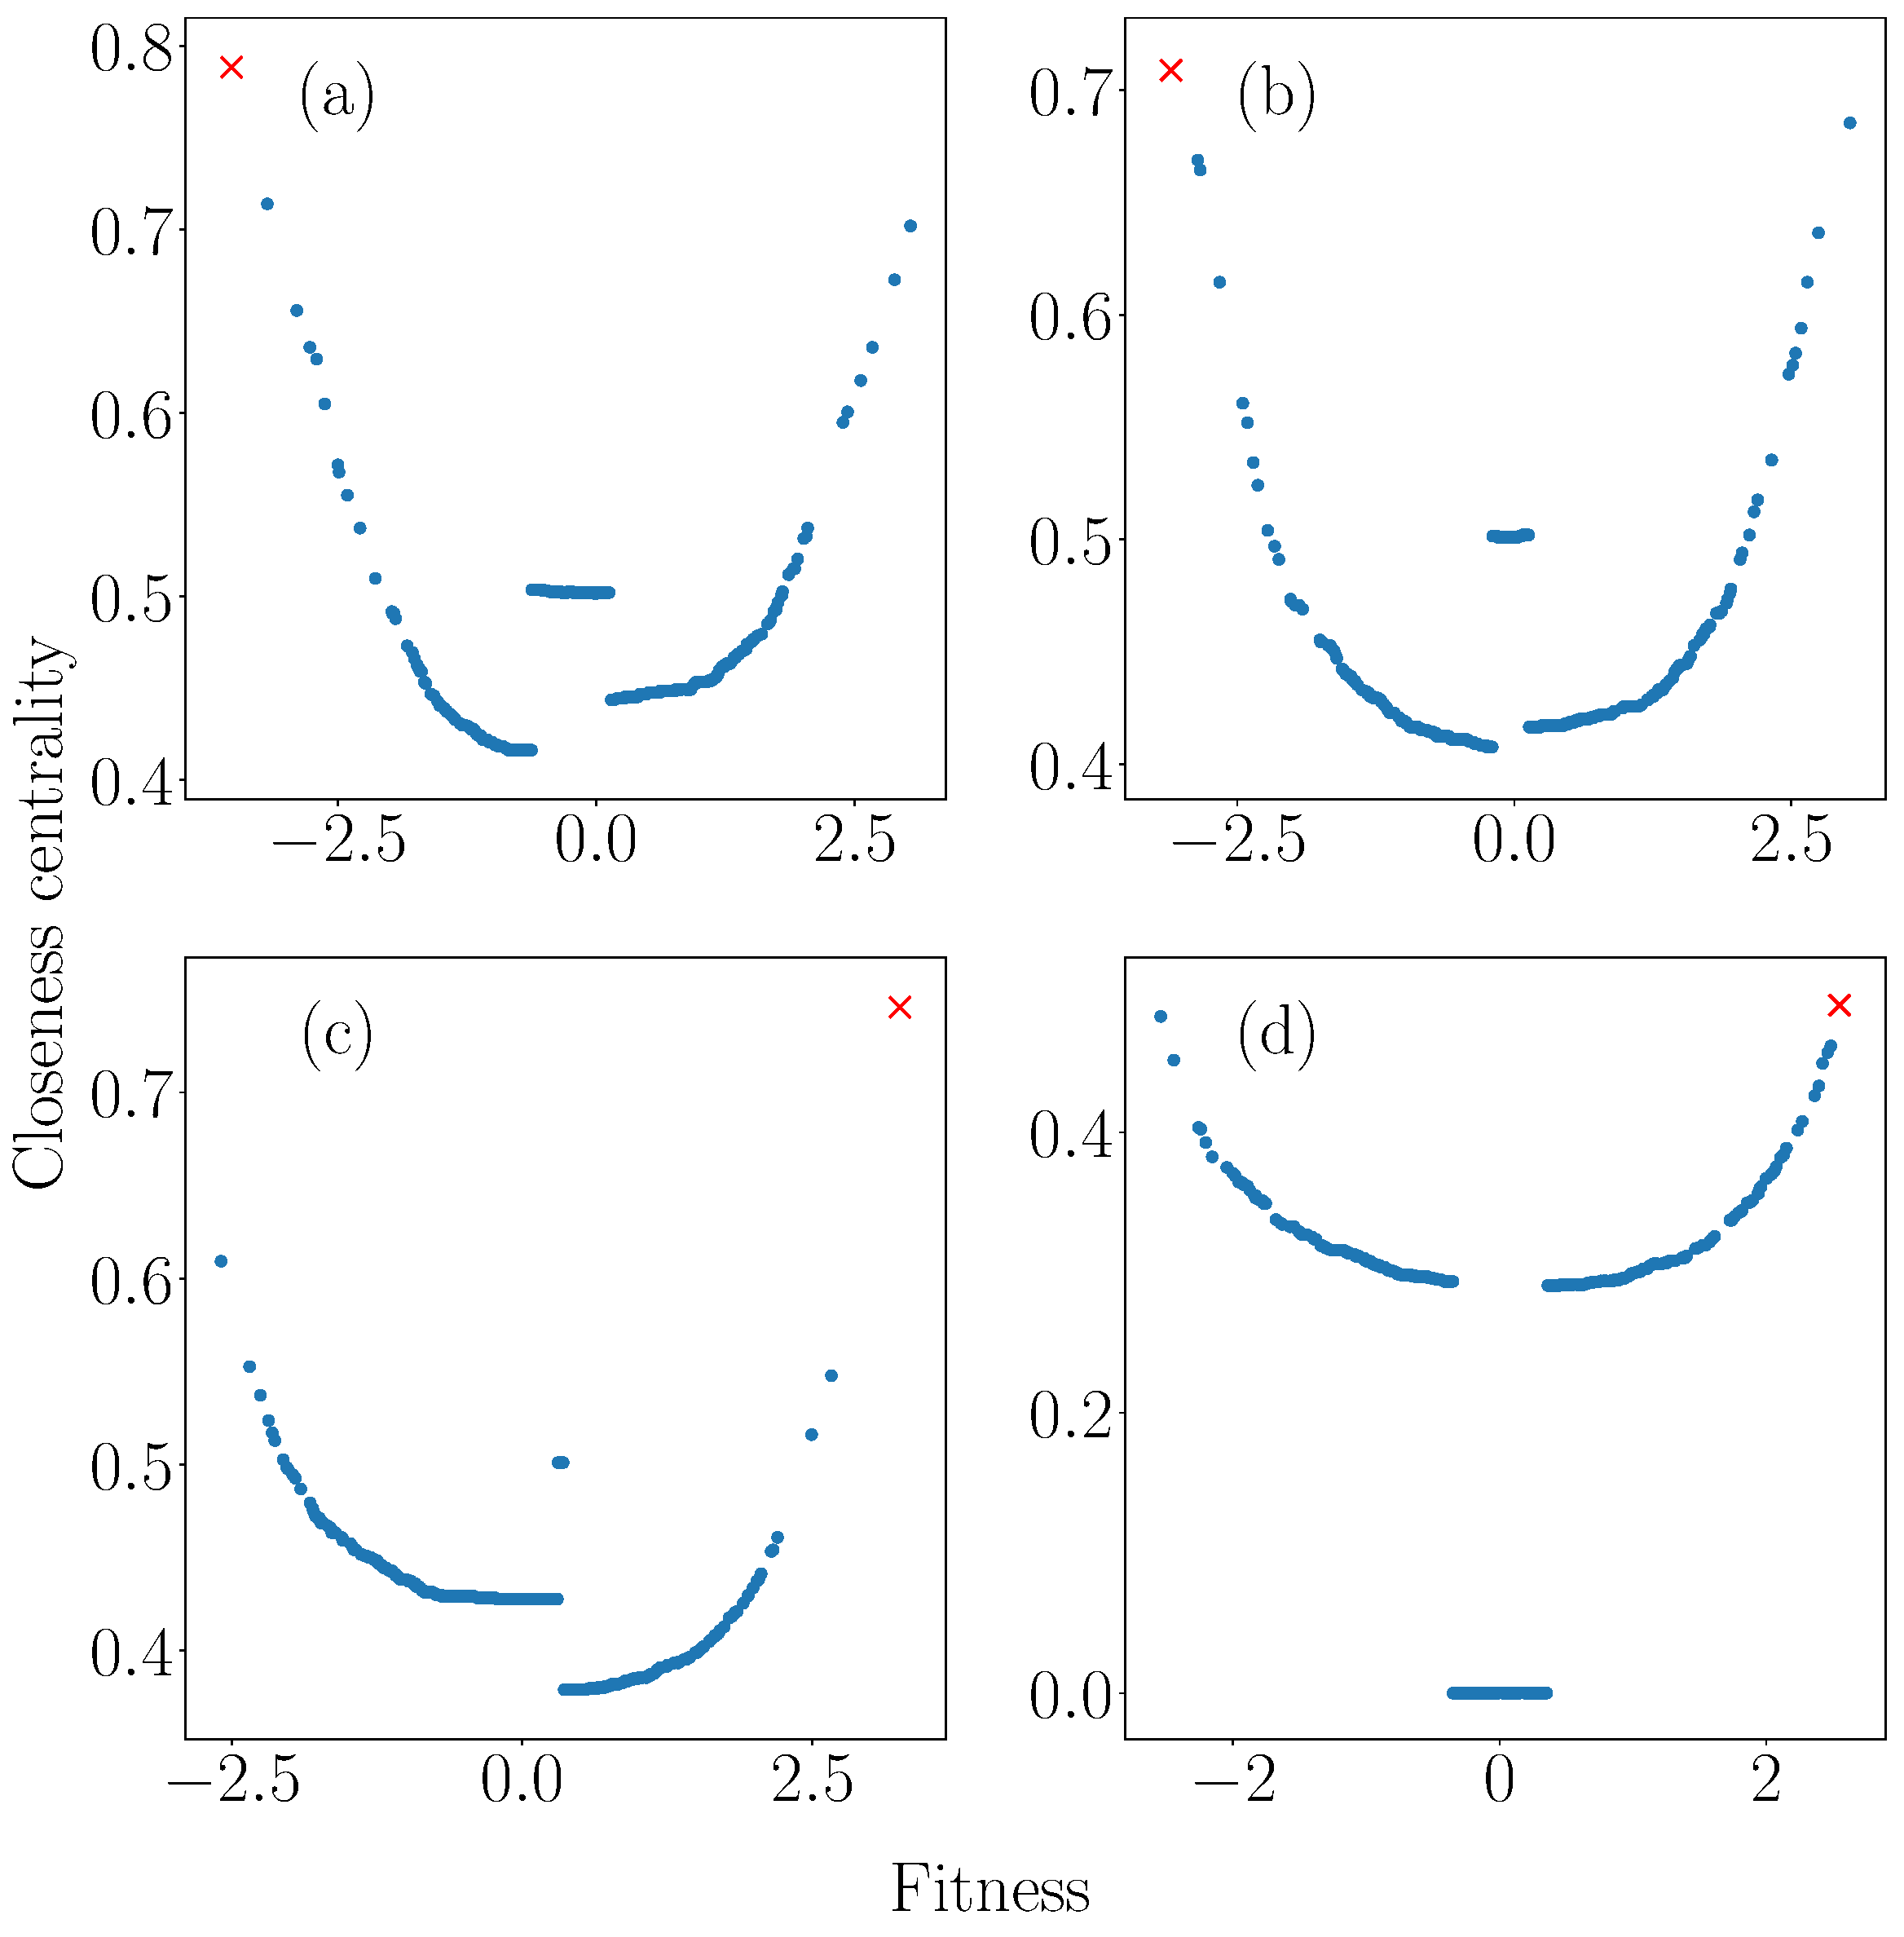
\includegraphics[width=0.8\linewidth]{geographic_beta_0_examples2_largerfont.pdf}
    \caption{Scatter plot of closeness centralities for nodes in $4$ instantiations of the geographical fitness model with decay parameter $\beta = 0$. All instantiations for $\beta = 0$ have similar scatter plots. The depicted instantiations illustrate common patterns. For each network, we highlight the node with the largest (in absolute value) fitness. In most scatter plots, we observe two large branches (on the left and right) and a small horizontal (or predominantly horizontal) curve between these two large branches. We refer to one branch as ``lower'' than the other if the lowest point of that branch is lower than the lowest point of the other branch. We observe that the left branch is lower when there is an extremum on the left (see the top-left and top-right panels) and that the right branch is lower when there is an extremum on the right (see the bottom-left plot). 
    }
    \label{fig:closeness_example}
\end{figure}


 

\begin{figure}
    \centering
    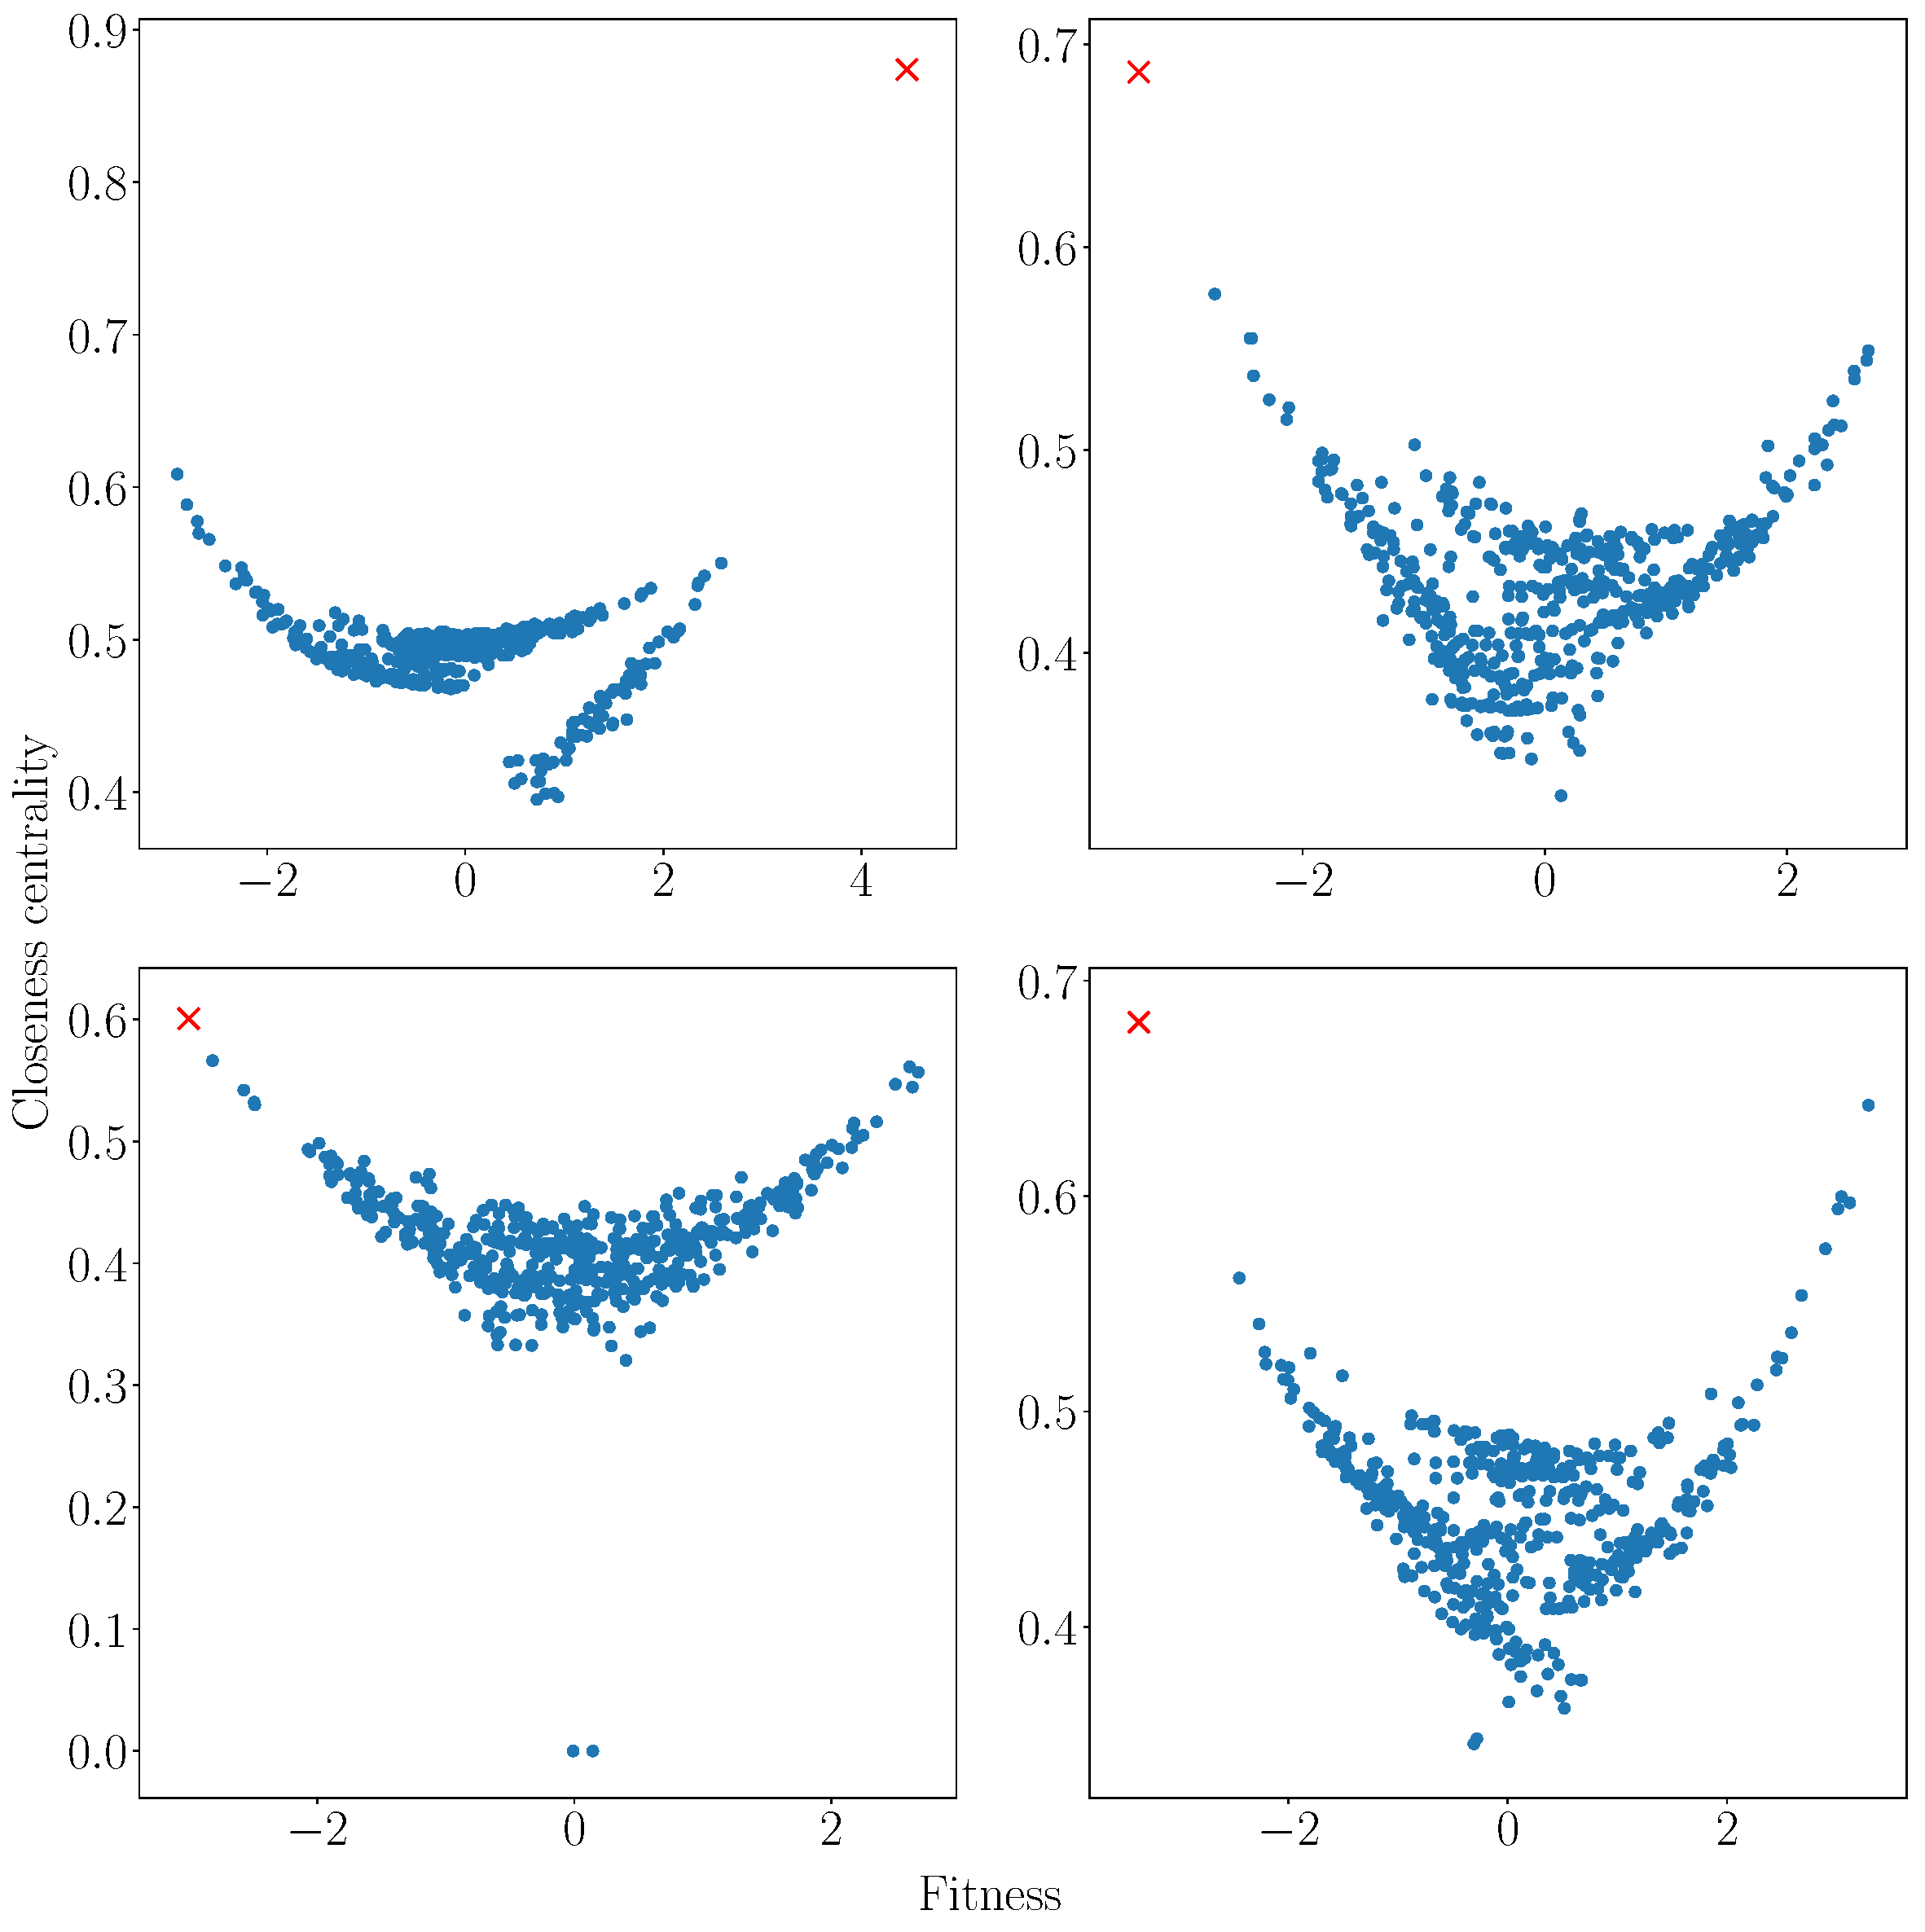
\includegraphics[width=0.8\linewidth]{geographic_beta_05_examples_largerfont.pdf}
    \caption{Scatter plot of closeness centralities for nodes in $4$ instantiations of the geographical fitness model with decay parameter $\beta = 0.5$. The depicted instantiations illustrate common patterns. For each network, we highlight the node with the largest (in absolute value) fitness. For this value of $\beta$, we do not always observe noticeable branches. (See the top-right, bottom-left, and bottom-right panels.) When there are noticeable branches in a scatter plot, they are usually accompanied by a node with a large absolute value of the fitness. (See the top-left panel.)
    }
    \label{fig:closeness_example_2}
\end{figure}


\begin{figure}
    \centering
    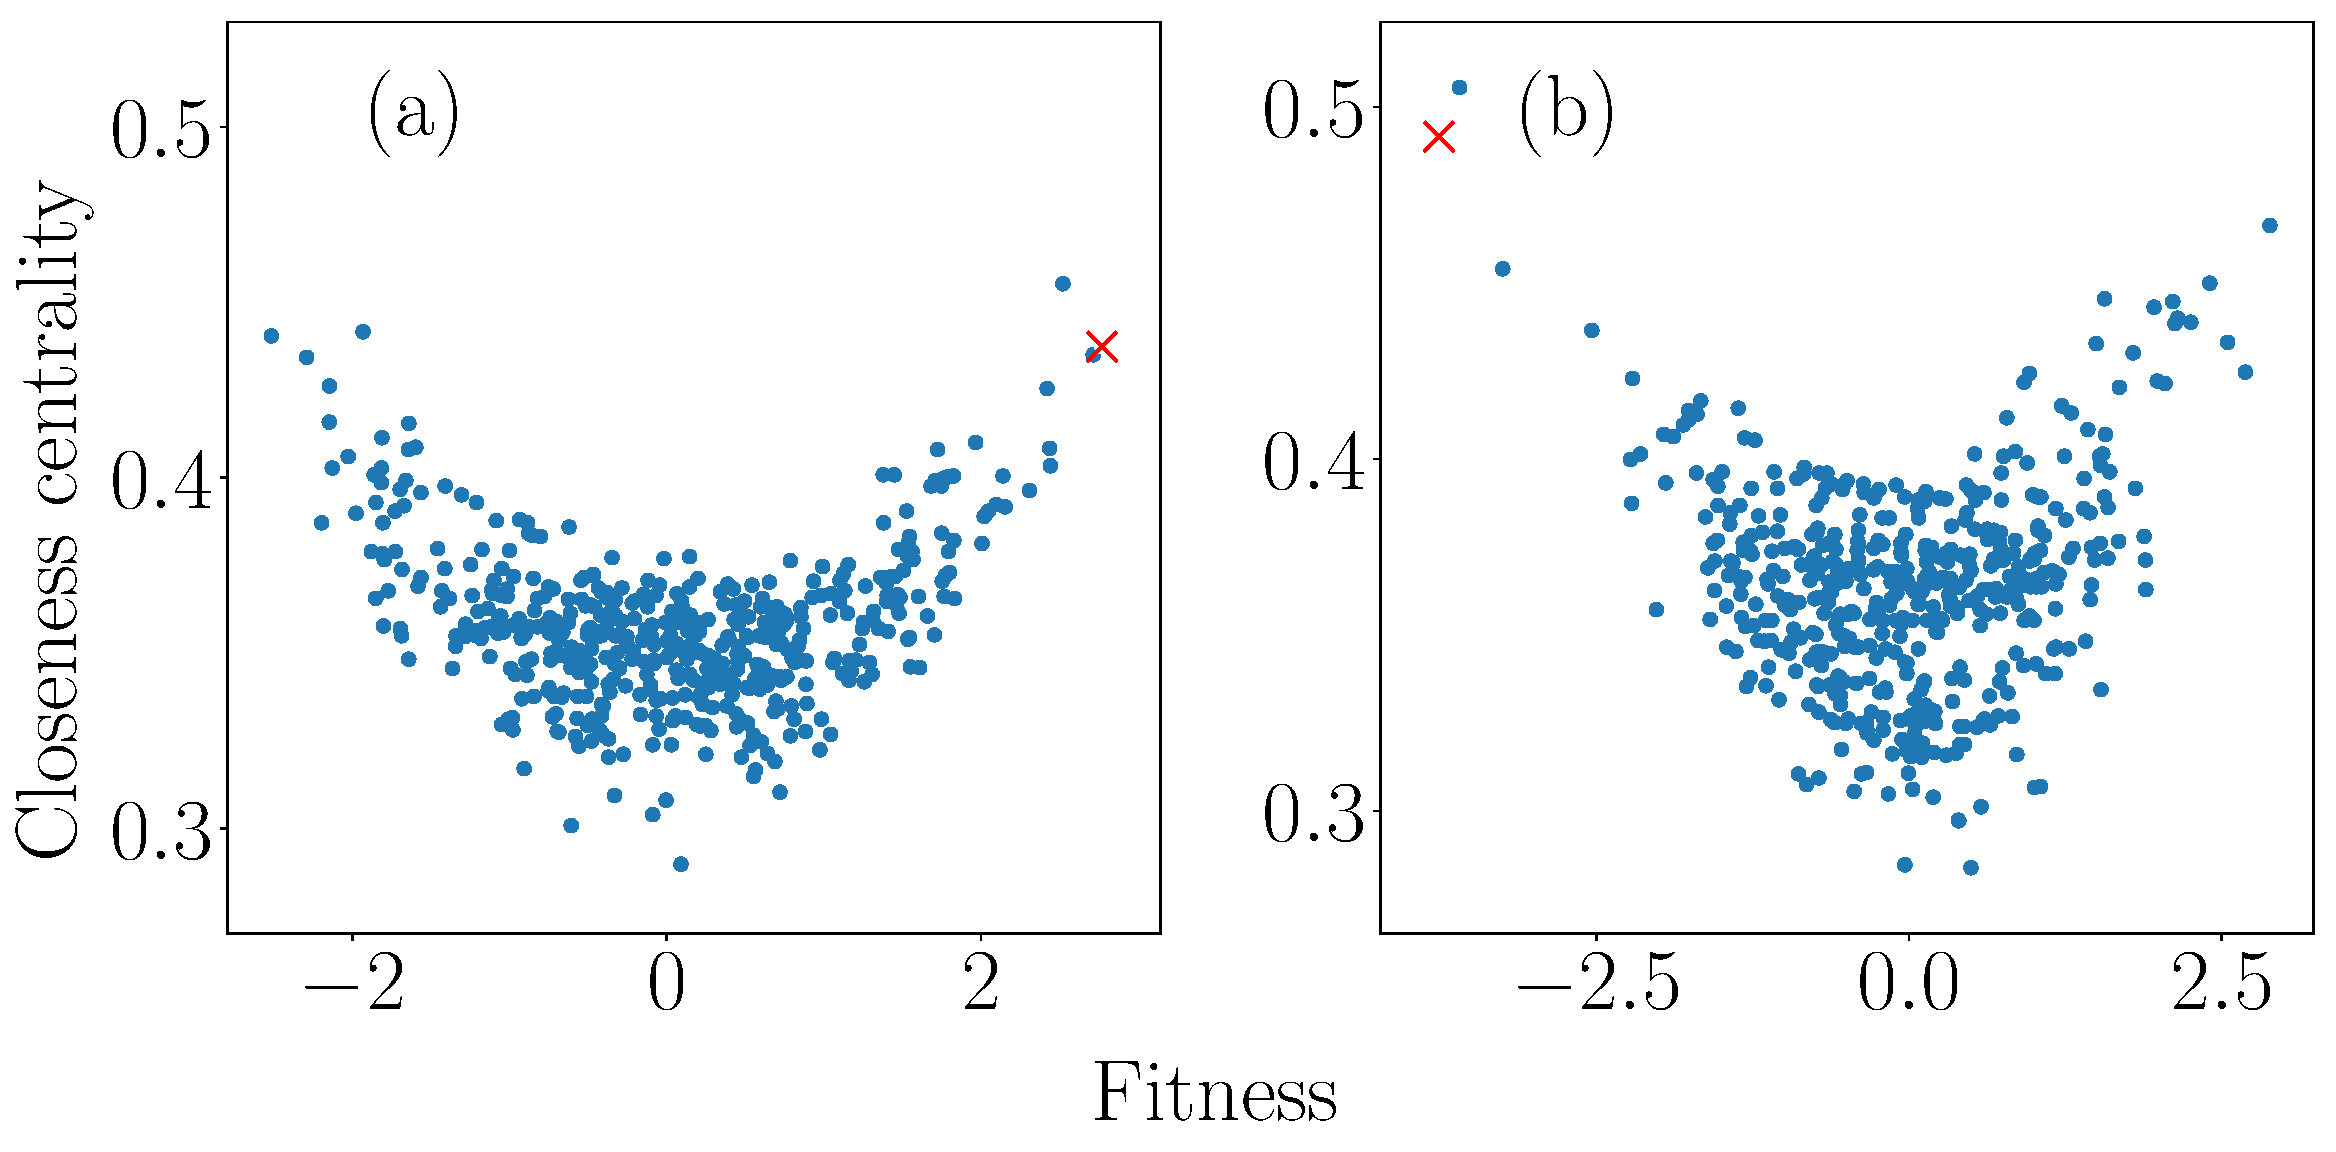
\includegraphics[width=0.8\linewidth]{geographic_beta_10_examples_largerfont.pdf}
    \caption{Scatter plot of closeness centralities for nodes in $2$ instantiations of the geographical fitness model with decay parameter $\beta = 1$.The depicted instantiations illustrate common patterns. For each network, we highlight the node with the largest (in absolute value) fitness. For this value of $\beta$, branches are almost never apparent in the scatter plots, even with extreme fitness value nodes (see the right plot), and the most extreme fitness value node is no longer always the one with the largest value of closeness centrality.
    }
    \label{fig:closeness_example_3}
\end{figure}


For $\beta = 0$, the closeness centralities of the nodes arise only from their intrinsic fitness values, as the model does not incorporate any spatial effects.
%considerations. 
In the scatter plots of fitness versus closeness centrality, we observe two large branches of values (see Fig.~\ref{fig:closeness_example}) in all networks from our $30$ instantiations. In these networks, the node whose fitness has the large absolute value (which we call the ``extremum'') is adjacent to all nodes in the network that have sufficiently different fitness; these nodes all belong to the other large branch, and the extremum acts as a shortcut to other nodes in the network.
%These nodes have increased closeness as the extremum acts as a shortcut to other nodes in the network. 

In these scatter plots, we also observe a small central curve between the two branches. It lies below the lowest point of the two branches (such as in the bottom-right scatter plot of Fig.~\ref{fig:closeness_example}) or above the nearby parts of both branches. This curve is below the branches when no nodes in the network have fitnesses with large enough absolute values, such that the nodes in the curve are not adjacent to any other node. {\color{red}Specifically, if the node with fitness closest to zero has a fitness value of $w_m$ and the extremum has a fitness value of $w_M$, then the small central curve is below the branches when $|w_M| < \theta - |w_m|$ ($\theta$ is approximately $2.9$ for $\beta = 0$).}
%when there are no nodes in the network with large enough absolute fitness, so these nodes are disconnected. 
%{\bf map: did I interpret the above sentence correctly? please confirm (or fix)}
Otherwise, they are adjacent to nodes with 
%have access to shortcuts from both 
very negative or very positive fitnesses. 

Extremum nodes still behave as shortcuts for $\beta = 0.5$, but the spatial constraints necessitate spatial proximity for nodes to be adjacent to other nodes, so the role of the extremum as a shortcut is less important, and some shortest paths go through other nodes. 
%{\bf map: I added the word "some" above; is that correct? otherwise, it was saying that all shortest paths go through other nodes; what is the correct situation here? we need to resolve this and make sure that what we write is precisely correct}
We show example scatter plots of closeness versus fitness for $\beta = 0.5$ in Fig.~\ref{fig:closeness_example_2}. In the top-left plot, for example, {\color{red}the presence of an extremum with very large fitness} still yields some branches in the scatter plot. However, in the other examples in this figure (and in most scatter plots from the $30$ instantiations), branches are less obvious. For $\beta = 1$ (and hence for larger values of $\beta$), branches are almost never apparent, as node fitnesses are less likely to determine whether two nodes are adjacent; instead, spatial effects become more prominent. We thereby see how spatial effects manifest in this geographical threshold model.
 
%This examination gives clues as to the behavior of the network characteristics as a function of $\beta$. The presence of shortcuts affects all of these characteristics, showing how spatial effects manifest in the geographical threshold model.

%%%%

\section{A Spatial Preferential-Attachment Model} \label{sec:ba-model}

\subsection{Prior research} \label{prior}

We now examine characteristics of a spatial generalization of the BA preferential-attachment model \cite{BA}. Such a spatial preferential-attachment model (SPA) was first introduced in \cite{SPA1} and explored further in \cite{SPA2, SPA3, SPA4}. 
%{\bf map: above: is it "this" one or "such" a model? from the text below, this isn't fully clear to me, but I am guessing "such"}
It starts with a seed network, with nodes located in $[0, 1] \times [0, 1] \subset \mathbb{R}^2$), at $t=0$. During each subsequent time step, one adds a new node and assigns its location
%coordinate assigned 
uniformly at random in the space. {\color{red}If a node is assigned the same location as an existing node, a different location is assigned uniformly at random.} New nodes are connected to $m$ existing nodes with probability 
\begin{equation}\label{spatialpreferential_prior}
    p(v_i,v_j) = \frac{k_j h(r_{i, j})}{\sum_l k_l h(r_{i,l})}\,,
\end{equation}
where $r_{i,j}$ is the Euclidean distance between nodes $v_i$ and $v_j$ and $h(r_{i,j})$ is the same as in (\ref{distance_equation}) (i.e., $h(r_{i,j}) = r_{i,j}^{-\beta}$). In \cite{SPA1}, this SPA was simulated on a 1D space. {\color{red} Based on numerical computations (taken as a mean over $10$ realizations), it appeared that it might have a power-law degree distribution $P(k)$ for $\beta < 1$ and a stretched exponential degree distribution for $\beta \geq 1$. For $\beta < 1$, the authors noted deviations from the corresponding power-law for small values of $k$. Based on the same simulations, the mean geodesic distance of the network appeared to scale logarithmically with the time steps for a wide range of $\beta$ (shown with up to $\beta = 5$). }
%{\bf map: was the above also numerical? this isn't precise enough}
%{\bf map: also, it says "diameter", so somehow the statement has to instead be a probabilistic one to be correct (as otherwise a single extremum can break it}
%{\bf andy: upon closer inspection I found the authors did in fact use mean geodesic distance, but just called it a network diameter}
{\color{red}References \cite{SPA2, SPA3} examined slight modifications to this SPA model, using the same connection probability (\ref{spatialpreferential_prior}) and generation procedure, but embedding the network in 2D space. }
Reference \cite{SPA2} assigned one new edge per incoming node and explored the distribution of edge lengths and the expected degree of a node born at time $t$.

%{\bf map: the previous paragraph is unclear: for example, it seems to switch back and forth as to whether there is one model or multiple different models that have been studied; it needs to be written more clearly}


Other spatial generalizations of the BA model have also been studied. In \cite{aiello, emmanuel}, for example, each node has a ``sphere of influence'' with size proportional to the node's in-degree. {\color{red}When a new node $v_t$ is added, if its location is inside the sphere of influence for an existing node, then $v_t$ is given a probability $p$ to create an edge to the existing node. As $t \rightarrow \infty$, the model exhibits power-law degree distribution and has a positive limit for the mean local clustering coefficient \cite{emmanuel}. }
%{\bf map: above: (1) need more clarity: which "limit" do you mean? this is clearly an asymptotic one, or else the statement about power laws wouldn't make sense; the above sentences (if it's going to be included at all) needs to be made more precise; (2) also, are you sure it's this clustering coefficient and not the global one? using the mean local clustering coefficient seems like choosing the more difficult object to work with}
%{\bf andy: they showed as $t \rightarrow \infty$, the mean local clustering coefficient had a positive limit, while the glocal clustering coefficient was non-negative (and positive with further restriction). This was shown analytically}

%In the model that was studied in \cite{geometric_preferential_attachment}, nodes are placed on a hyperbolic disk based on the position of existing nodes. The family of networks shows positive clustering, power-law degree distribution, and soft communities in the asymptotic limits.
%{\bf map: the above sentence is problematic for similar research as prior ones: (1) which precise limit is this? (2) "positive clustering": the word 'clustering' could mean many things, so what exactly do you mean by this; (3) what are "soft communities"? I have no idea whatsoever what this means; this needs to be defined in a precise way if we are going to use these terms (and is this something that is even meant in a precise way?) [note: you appear to be adopting statements from these papers without being sufficiently careful as to their precision or accuracy; you need to be more careful about how you write statements from previous papers into your own work]}
%{\bf andy: I opted to remove discussion of this reference entirely, it felt less related (very different model formulation) to the other models discussed in this paper}


\subsection{Description of our SPA model}

{\color{red}In the present paper, in contrast to the SPA models in \cite{SPA1,SPA2,SPA3}, which use a connection probability given by equation (\ref{spatialpreferential_prior}), we instead use a connection probability function of}
\begin{equation} \label{spatialpreferential}
    p(v_i,v_j) = \frac{k_j}{\sum_l k_l}h(r_{i,j})\,.
\end{equation}
The intuition behind our choice is that the ``popularity'' of a node (given by its relative degree in a network) is independent of its distance from another node. This allows us to transform an existing non-spatial PA model (such as the BA model) into a spatial variant by multiplying the probability that an edge forms by a deterrence function $h(r)$. {\color{red}We do not consider self-edges or multi-edges. The probability that an incoming node $v_t$ at time step $t$ forms an edge with any other node in the network (after normalizing this probability such that it sums to $1$) is thus
\begin{equation} \label{spatialpreferential_normalized}
p(v_t, v_j) = \frac{p(v_t, v_j)}{\sum\limits_{\substack{j < t \\ \{j  |  v_j \not\in N(v_t)\}}} p(v_t, v_j)},
\end{equation}
where $N(v_t)$ is the set of nodes to which $v_t$ is adjacent (i.e., its neighborhood). When implemented in an algorithm, the edges are assigned one at a time.}

We assign a location uniformly at random in $[0, 1] \times [0, 1]$ to each node as we add it to the network. 
We start our network with a seed that consists of a $10$-clique (each node in this $10$-clique is assigned a location uniformly at random). At each time step, we add a new node $v_i$ with $m=5$ stubs (i.e., ends of edges), and we connect each of these stubs to an existing node in the network with probability equal to \eqref{spatialpreferential_normalized}.
Consequently, nodes with larger degrees are more likely to accrue more connections and incoming nodes are more likely to connect to nearby nodes than to ones that are farther away. All edges are undirected and unweighted. 

For computations, we consider decay parameters of $\beta \in \{ 0, 1, 2, 3, 4\}$, and we examine $10$ instantiations of our model for each value of $\beta$.
We simulate each instantiation of our model for $T$ time steps, and we consider $T \in \{300, 1000, 3000, 10000\}$ {\color{red}(note that these will respectively have $n \in \{310, 1010, 3010, 10010\}$ nodes due to the $10$ nodes in the seed network).} Because each node adds $5$ edges to a network, it follows that $\langle k \rangle \rightarrow 10$ as $T \rightarrow \infty$.


%%%%%

\subsection{Computational results}




\begin{figure}
    \centering
    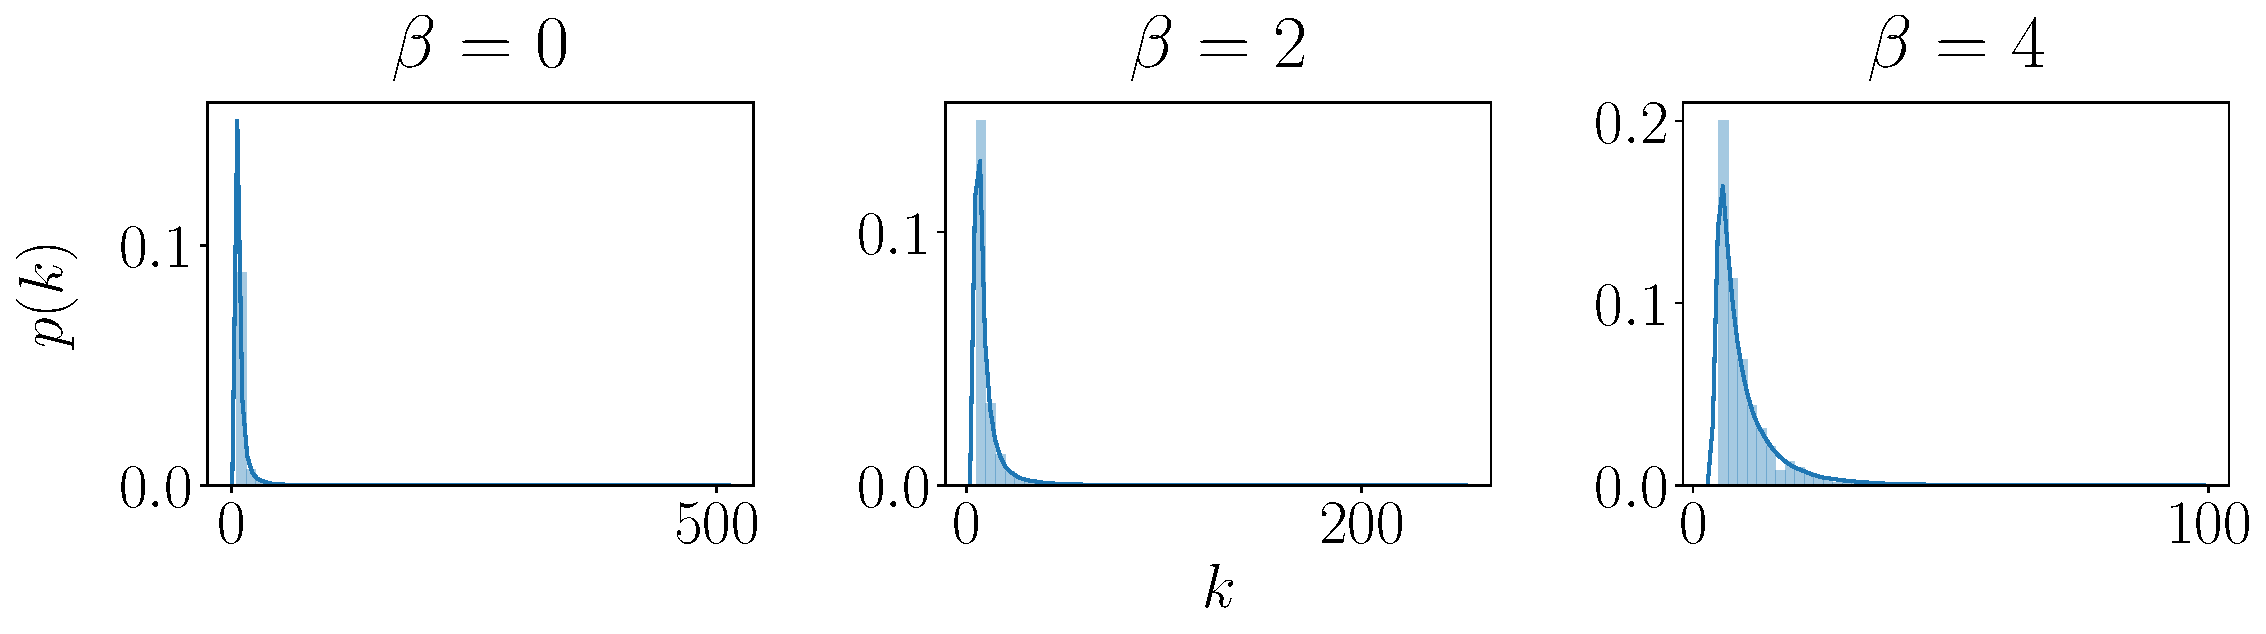
\includegraphics[width=1.0\linewidth]{preferential_attachment_degree_distribution.pdf}
    \caption{Degree distributions for single instances of our SPA model for $T=10000$ time steps. From left to right, we show examples for $\beta = 0$, $\beta = 2$, and $\beta = 4$.
    }
\end{figure}




\begin{figure}
    \centering
    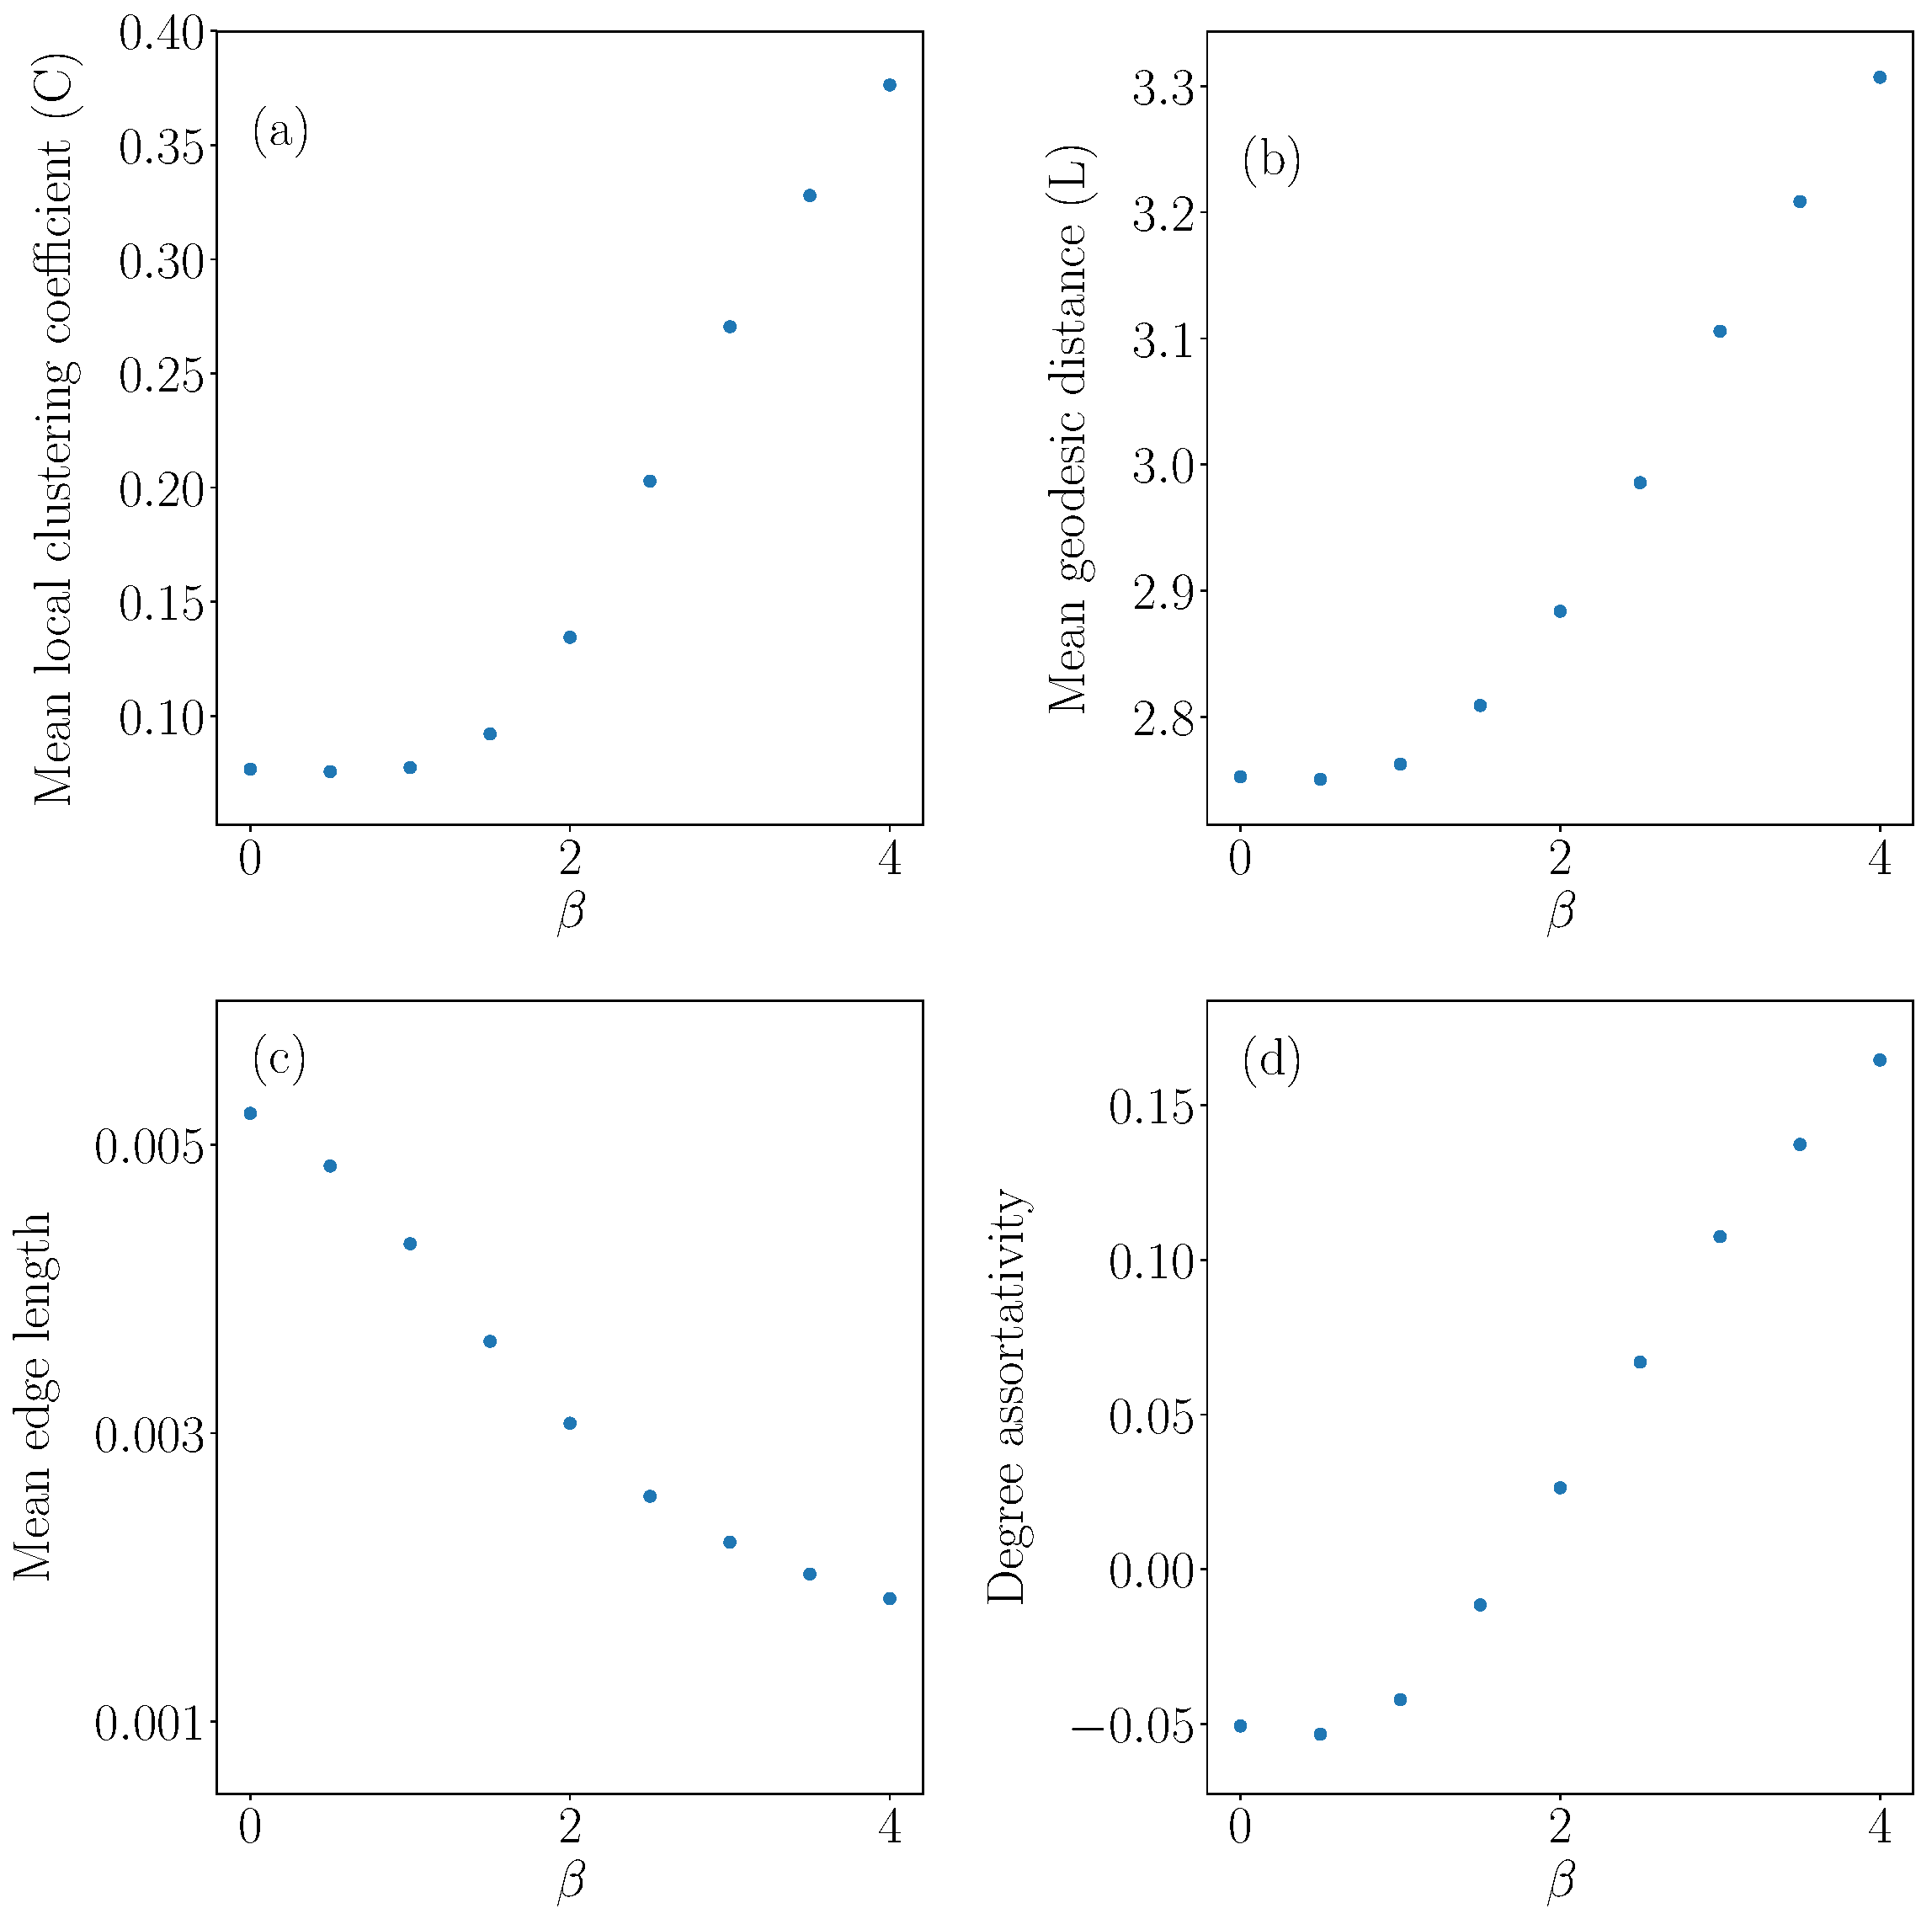
\includegraphics[width=1.0\linewidth]{preferential_attachment_metrics.pdf}
    \caption{Some characteristics of the networks from our SPA model for different values of the spatial decay parameter $\beta$ for networks with $n=10010$ nodes, $m=5$ edges for each new node as we add it, and $10$ instantiations of our model. We show computations of (a) mean local clustering coefficient, (b) mean geodesic distance, (c) mean edge length, and (d) degree assortativity.
    }
\end{figure}


\begin{figure}
    \centering
    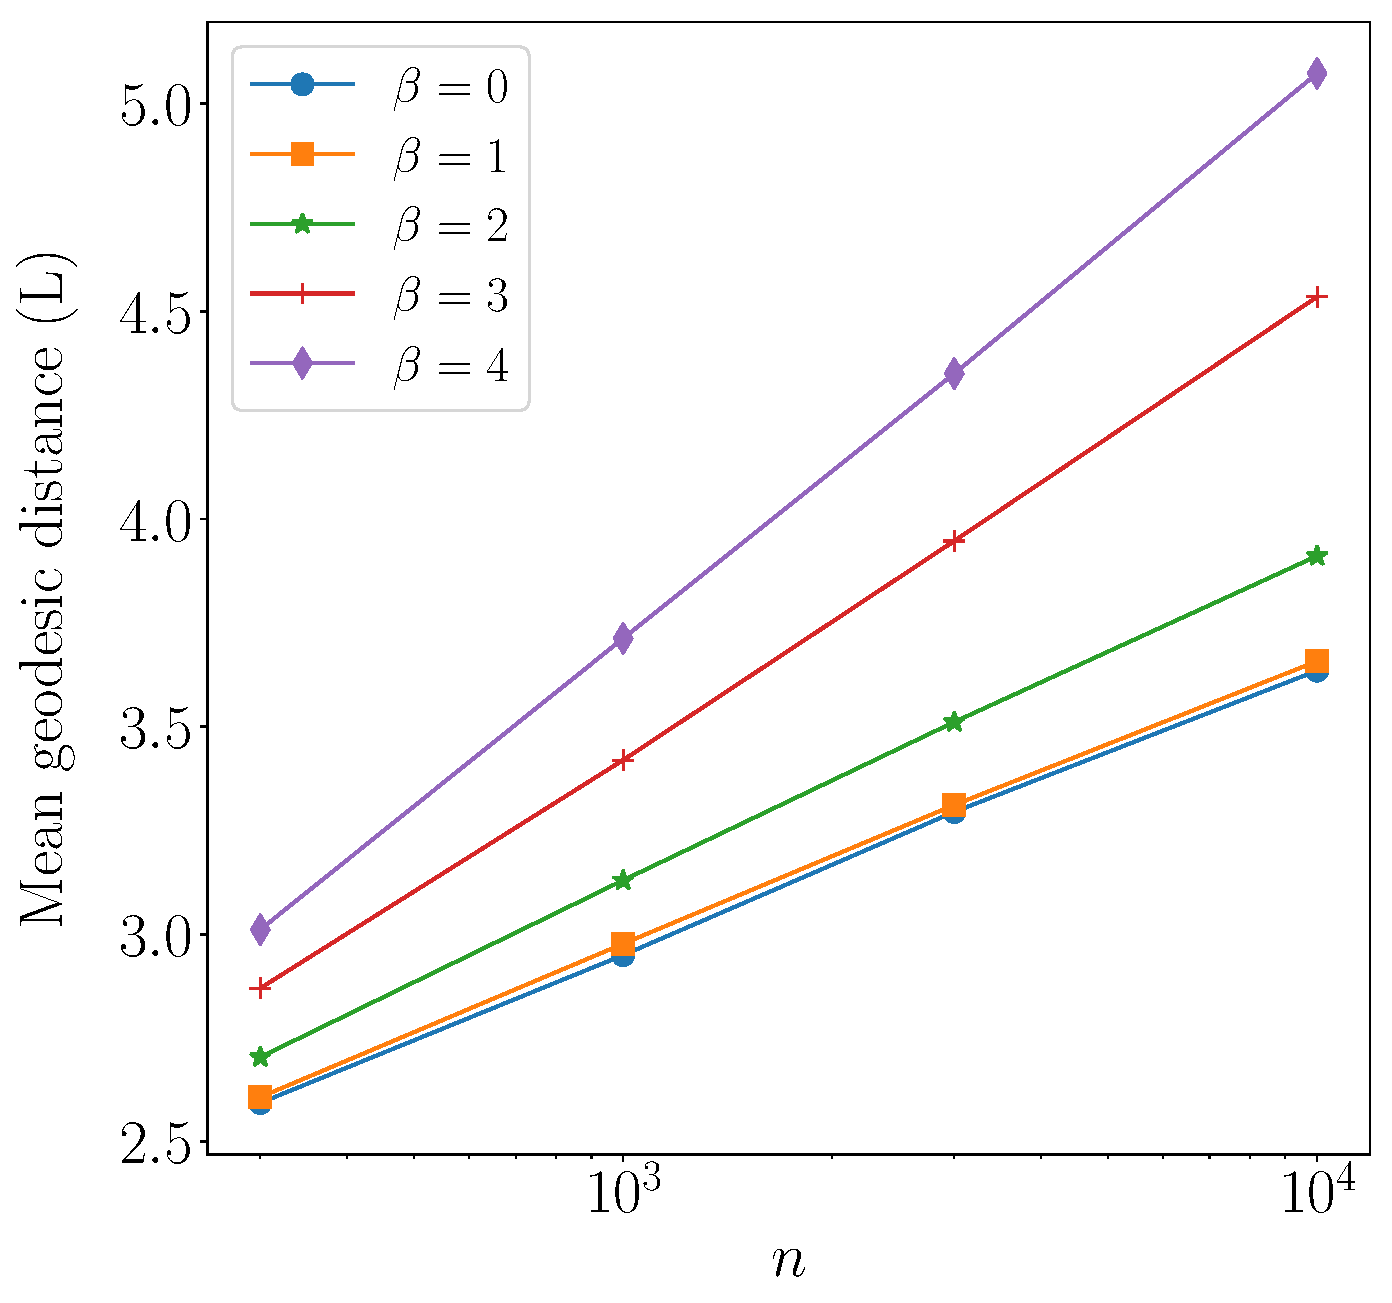
\includegraphics[width=0.75\linewidth]{PA_log_geodesic.pdf}
    \caption{Mean geodesic distance of our SPA networks as a function of the number of nodes in a network for several values of the spatial decay parameter $\beta$.
    %, with $\beta \in {0, 1, 2, 3, 4}$. 
    We show the number $n$ of nodes shown on a logarithmic scale. Each point in the plot represents a mean of the mean geodesic distances over $10$ instantiations of our model for each value of $n$ and $\beta$.
    }
    \label{fig:PA_geodesic}
\end{figure}




\begin{figure}
    \centering
    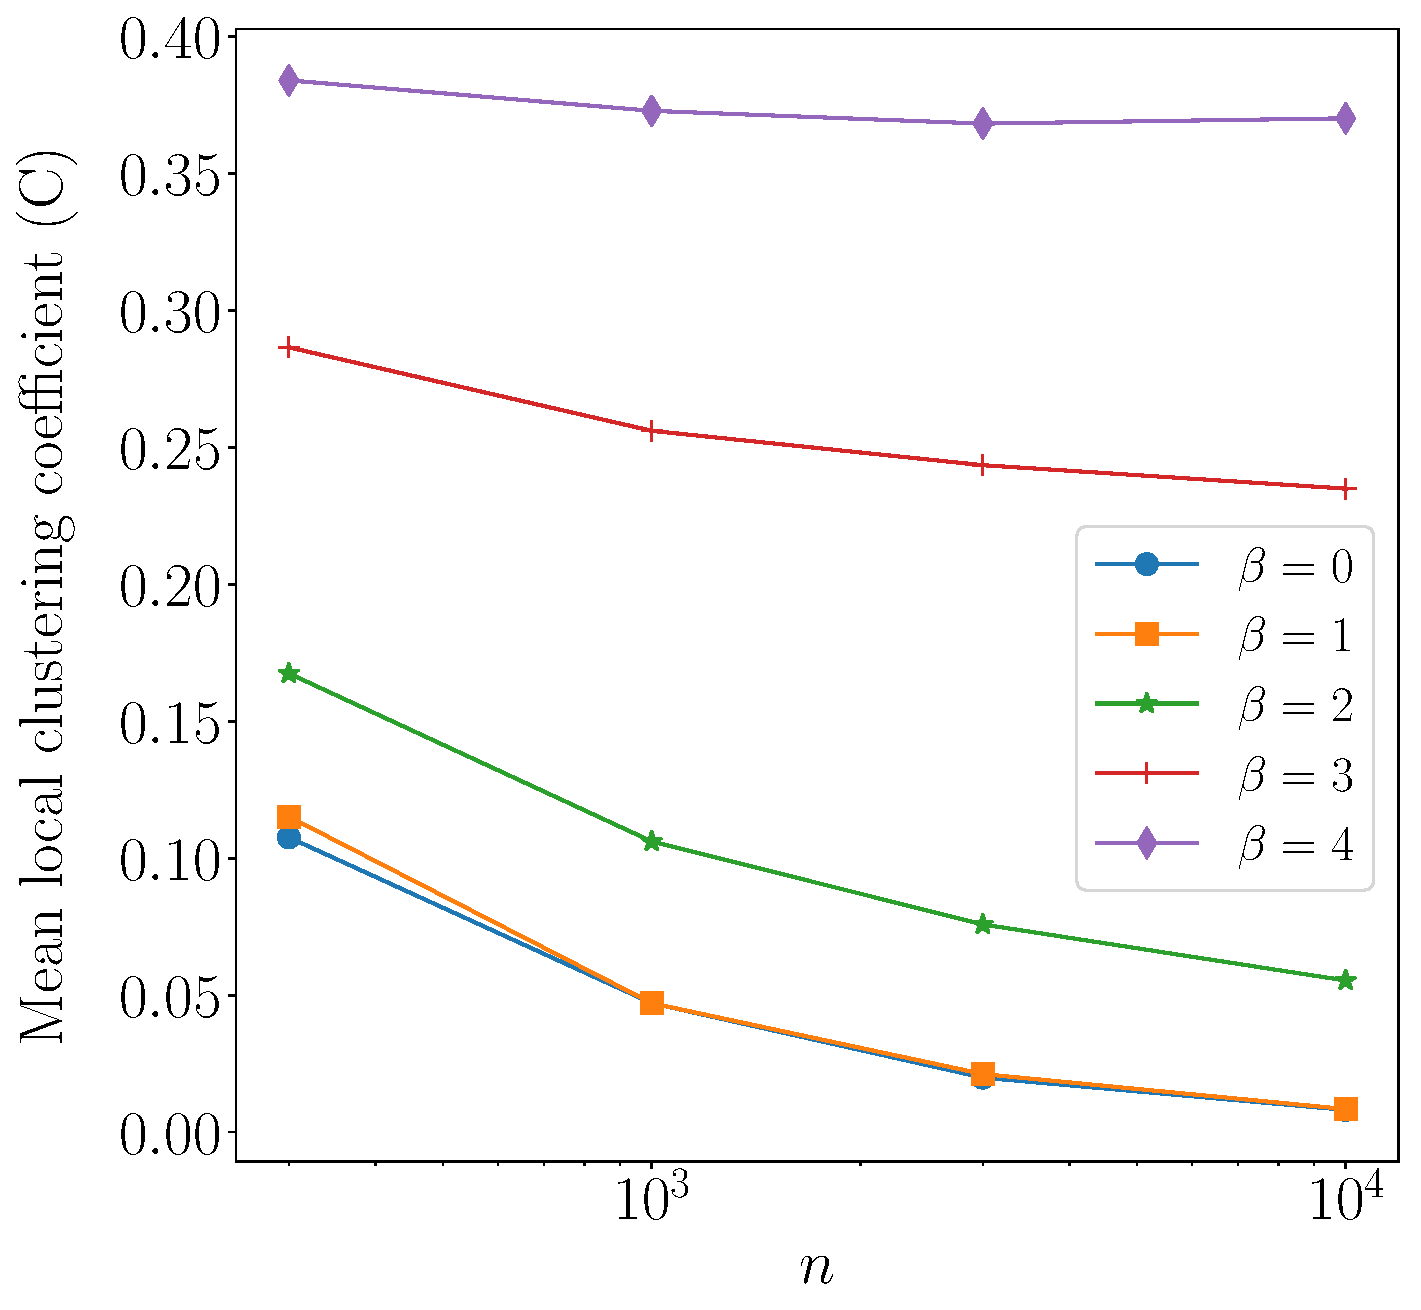
\includegraphics[width=0.75\linewidth]{PA_log_clustering.pdf}
    \caption{Mean local clustering coefficients of our SPA networks as a function of the number of nodes in a network for several values of the spatial decay parameter $\beta$.
    %, with $\beta \in {0, 1, 2, 3, 4}$. 
    We show the number $n$ of nodes on a logarithmic scale. Each point in the plot represents a mean of the mean local clustering coefficients over $10$ instantiations of our model for each value of $n$ and $\beta$.
    }
    \label{fig:PA_clustering}
\end{figure}


As with the GF model, we calculate the mean local clustering coefficient, geodesic distance, edge length, and degree assortativity. (See Section \ref{sec:fitness_model} for definitions of these quantities.) In our SPA model, we observe the {\color{red}same general trends in these quantities as we increase the spatial decay parameter $\beta$ as we observed in the GF model.} Specifically, the mean local clustering coefficient, geodesic distance, and degree assortativity increase as we increase $\beta$; and the mean edge length decreases as we increase $\beta$.

We examine in more detail how the mean geodesic distance (see Fig.~\ref{fig:PA_geodesic}) and mean local clustering coefficient (see Fig.~\ref{fig:PA_clustering}) change as a function of the number of nodes for SPA networks. 
%Note that these figures have a logarithmic scaling for $n$. 
In Fig.~\ref{fig:PA_geodesic}, for spatial decay parameter values of $\beta \in \{0, 1, 2, 3, 4\}$, the mean geodesic distance seems to increase logarithmically scaling with the number $n$ of nodes according to numerical simulations. This is consistent with the observations for a 1D SPA in \cite{SPA1}, which found {\color{red}mean geodesic distance to have logarithmic scaling with respect to $n$ based on numerical simulations. }

%{\bf map: see my previous comment about diameter; the statement above needs to be made more precise; there must be some kind of probabilistic statement in what they found (and was it only numerically?)}

In Fig.~\ref{fig:PA_clustering}, we see for $\beta \in \{0,1,2\}$ that the mean local clustering coefficient decays sharply for progressively larger $n$, and it is possible that it may approach $0$ as $n \rightarrow\infty$.
Meanwhile, for $\beta=4$ and $\beta=3$, we do not observe such sharp decay, at least for the examined values of $n$.
Our numerics suggest the possibility that it may be the case that there is a value $\beta_c$ such that $\beta > \beta_c$, one obtains a positive mean local clustering coefficient in the limit that $n \rightarrow \infty$.

%{\bf map: I have changed the above paragraph very significantly, as I found significant issues with it}


%%%%%

\section{A Spatial Configuration Model} \label{sec:configuration_model}

We now generalize a configuration model \cite{fosdick, newman2018} to incorporate spatial considerations. Configuration models are among the most important random-graph models, as they are used frequently as reference models (including as null models in community detection \cite{community1, community2}) for a large variety of network analyses. We envision that spatial analogs of configuration models will be similarly helpful for spatial networks.

%%%%

\subsection{Description of the model}

{\color{red}Our goal in developing a spatial configuration model is to preserve the degree sequence of an input network, randomizing the adjacency according to some rule that incorporates spatial embedding. Specifically, nodes are embedded in a latent space and assigned a number of edge stubs according to the degree sequence of the input network. Then, edge stubs are connected (in a process similar to a non-spatial configuration model \cite{fosdick}), but rather than selecting edge stubs uniformly at random, we preferentially connect stubs that are spatially close. }

%Our goal in developing a spatial configuration model is to preserve the degree sequence of an input network, embed its nodes in a latent space, and then configure the adjacency of the network to incorporate the new spatial embedding. 
%{\bf map: "then configure the adjacency of the network to incorporate the new spatial embedding": what do you mean by this? we need to be clearer with this part of the sentence}
%There are many possible ways to follow the above approach. For example, one can embed nodes in any sort of space with different randomizations, and one incorporate a spatial embedding in numerous ways. 
%{\bf map: "one can embed nodes in any sort of space with different randomizations": I have no idea what you mean by this phrase; this needs to be rephrased}

{\color{red}We must make specific choices for this process. We must choose how to assign node locations. They can be assigned uniformly at random, or according to a different randomization. If the input network is embedded in space and includes node locations, we can also consider leaving the node locations unmodified. We must also choose how to bias stub selection to connect spatially close stubs. In our model, we use a deterrence function in a similar fashion as the previous SPA and GF models. }Our procedure is the following:
\begin{enumerate}
    \item For each node, assign a new location, which we choose uniformly at random, in $[0, 1] \times [0, 1]$.
    \item To each node $v_l$ with degree $k_l$, assign $k_l$ stubs to it. We denote the number of unmatched stubs for a node $v_l$ at time step $t$ by $u(v_l, t)$.
    \item Choose a stub from step (2) uniformly at random. We label its associated node as $v_i$.
    \item Choose a second stub with a probability proportional to $h(r_{i,j})$. That is, select a stub from node $v_j$ with probability
   \begin{equation*}
        p(v_i, v_j, t) = \frac{u(v_j, t)h(r_{i,j})}{\sum_{l \neq i} u(v_l, t)h(r_{i,l})} \,.
    \end{equation*}
    \item Connect the two stubs from steps (3) and (4) to each other with an undirected, unweighted edge. 
    \item Repeat steps (3)--(5) until all we have matched all stubs to form edges.
\end{enumerate}

Because $r_{i,j}$ is independent of the time step, we can make the above process more efficient by calculating the pairwise Euclidean distance between all node pairs in a network (there are $O(n^2)$ such pairs to calculate) and store it for reuse in each stub-choosing step. After this, the algorithm takes $O(|E| n)$ time to run, where $E$ denotes the set of edges and $|E|$ is the number of edges.

In formulating a spatial configuration model, one needs to decide whether to allow multi-edges and/or allow self-edges. {\color{red}Since $h(r_{i,i}) = 0^{-\beta}$ does not have a well-defined value for positive values of $\beta$, we choose not to consider self-edges to get around this issue. We allow multi-edges.}
%{\bf map: is not having a well-defined value quite the reason that we don't allow it, or is it something slightly different?}

There are also many other types of spatial configuration models that one can develop. For example, one can randomize the positions of nodes while preserving the adjacency matrix of the network. 
%{\bf map: I don't know what you mean by "connectivity" in the above sentence; this needs to be clarified}

As with non-spatial configuration models \cite{fosdick}, choices regarding the implementation of the spatial configuration process should depend on the application and question of interest. One common application of a configuration model is to use it as a null model in community detection \cite{forcechains, community1, community2}, where the exact choice of the null model greatly affects which communities are detected. 


%%%%%

\subsection{Computational results}

%For demonstration of this procedure, w
To illustrate the properties of our spatial configuration model, we start by generating a standard BA network. The seed network for the BA network is a $10$-clique, each new node has $m=5$ stubs, and we grow the network for a total of $T=1000$ time steps (such that the final network has $n=1010$ nodes). We then use the degree sequence from this network as the degree sequence for networks that we construct from our spatial configuration model. {\color{red}Note that a new BA network is generated for each application of the spatial configuration model.}

\begin{figure}
    \centering
    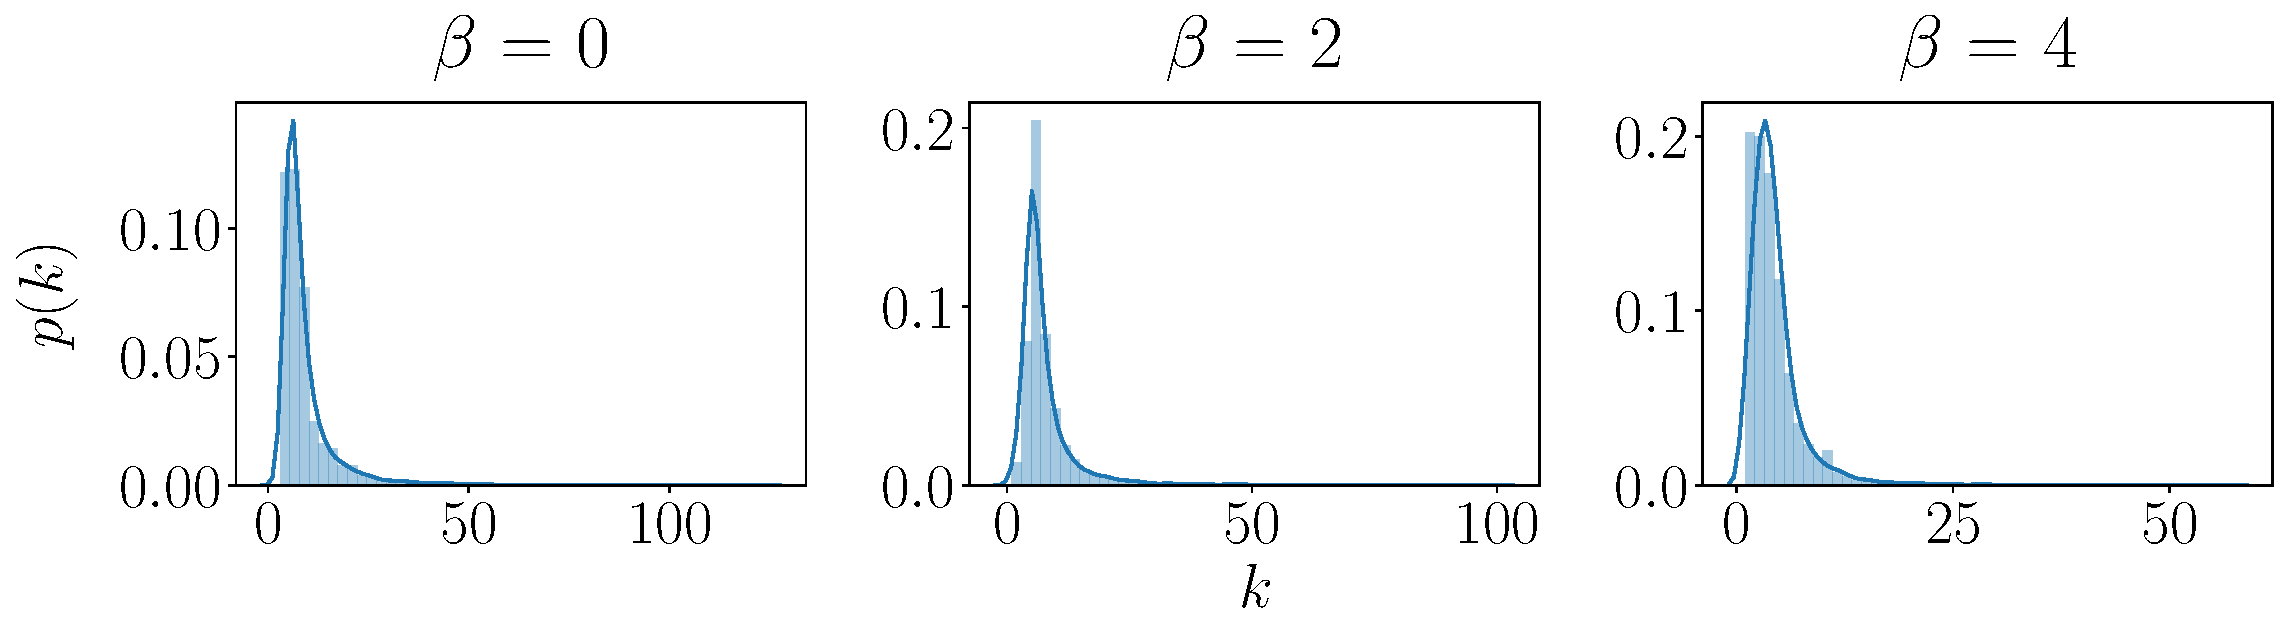
\includegraphics[width=1.0\linewidth]{spatial_configuration_degree_distribution.pdf}
    \caption{Degree distributions for single instances of the spatial configuration 
     model, with degree sequence given by a BA network with $n=1010$ nodes and $m=5$ new edges for each node that we add after the seed, for spatial decay parameters of $\beta = 0$, $\beta = 2$, and $\beta = 4$.
     }
\end{figure}


\begin{figure}
    \centering
    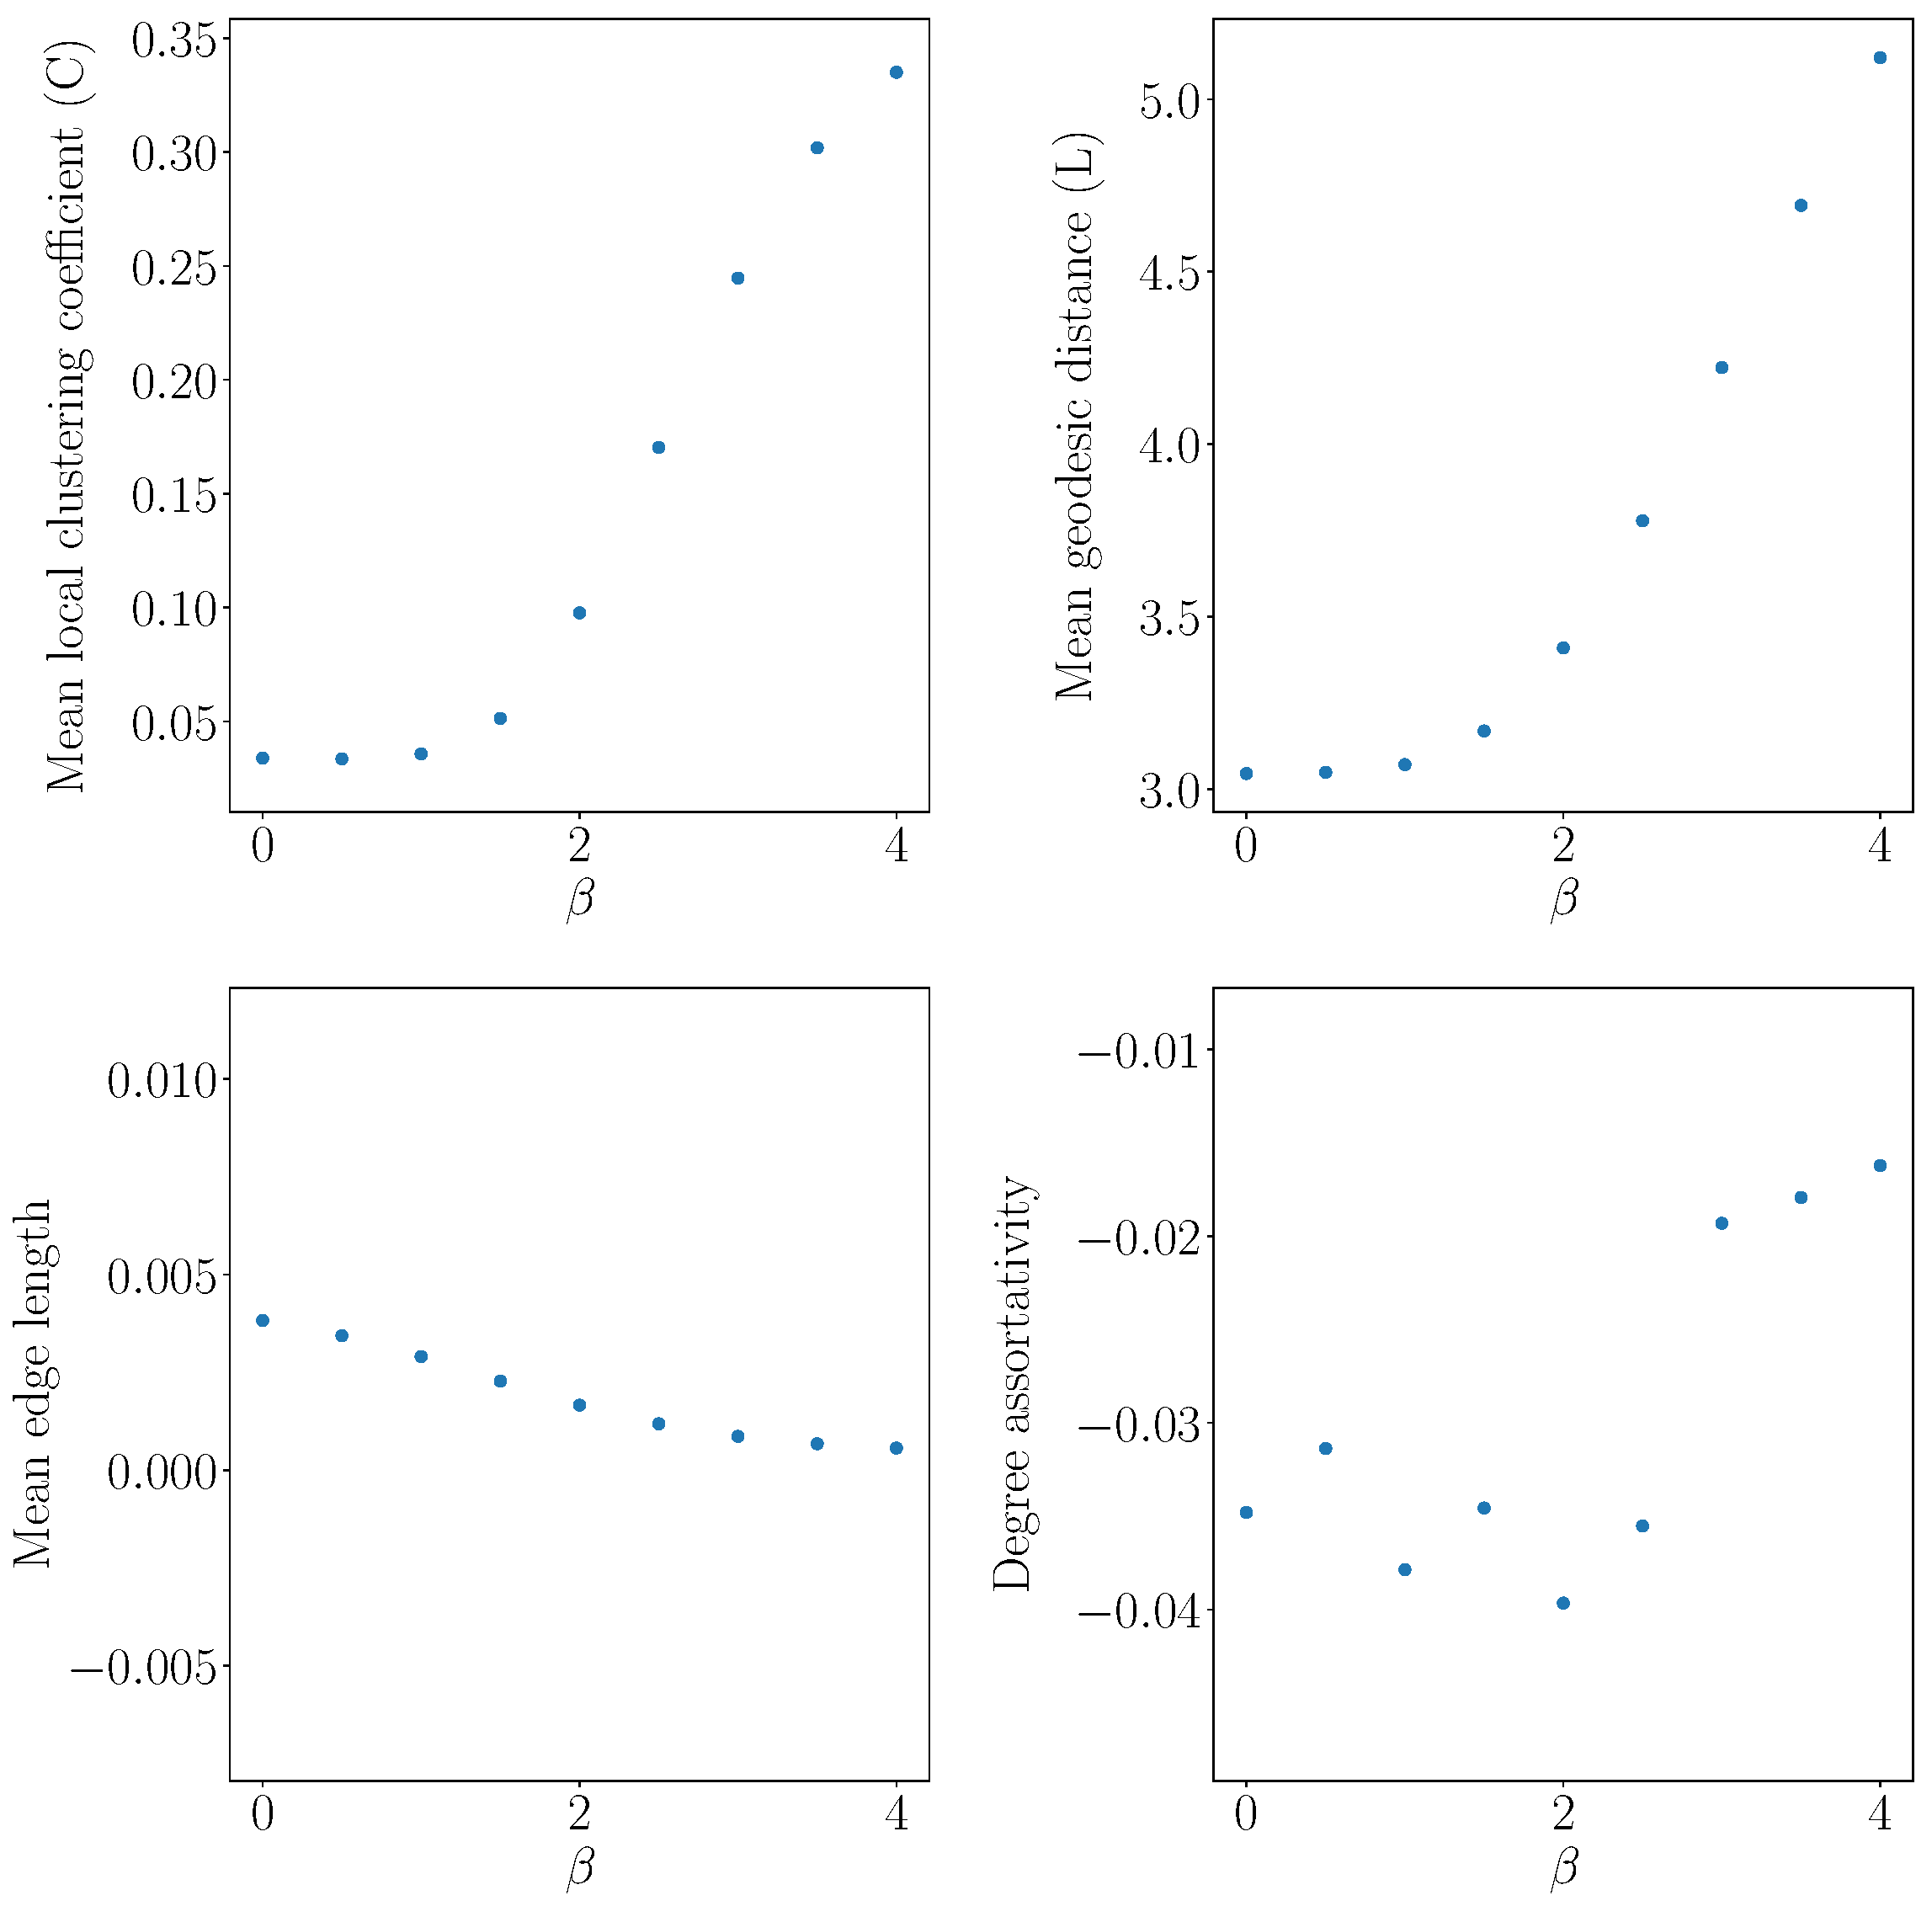
\includegraphics[width=1.0\linewidth]{spatial_configuration_metrics2.pdf}
    \caption{Some characteristics of the networks from our spatial configuration-model networks for various values of $\beta$. We use a degree sequence given by a BA model with $n=1010$ nodes and $m=5$ new edges for each node that we add after the seed. {\color{red}A new BA network is generated for each instantiation. }We take means of the network characteristics over $30$ instantiations of our model.
    %{\bf map: using the same exact BA network in each one, or is it 30 different BA networks? this needs to be specified}
     We show computations of (a) mean local clustering coefficient, (b) mean geodesic distance, (c) mean edge length, and (d) degree assortativity.
    }
    \label{fig:spatial_configuration_metrics}
\end{figure}


\begin{figure}
    \centering
    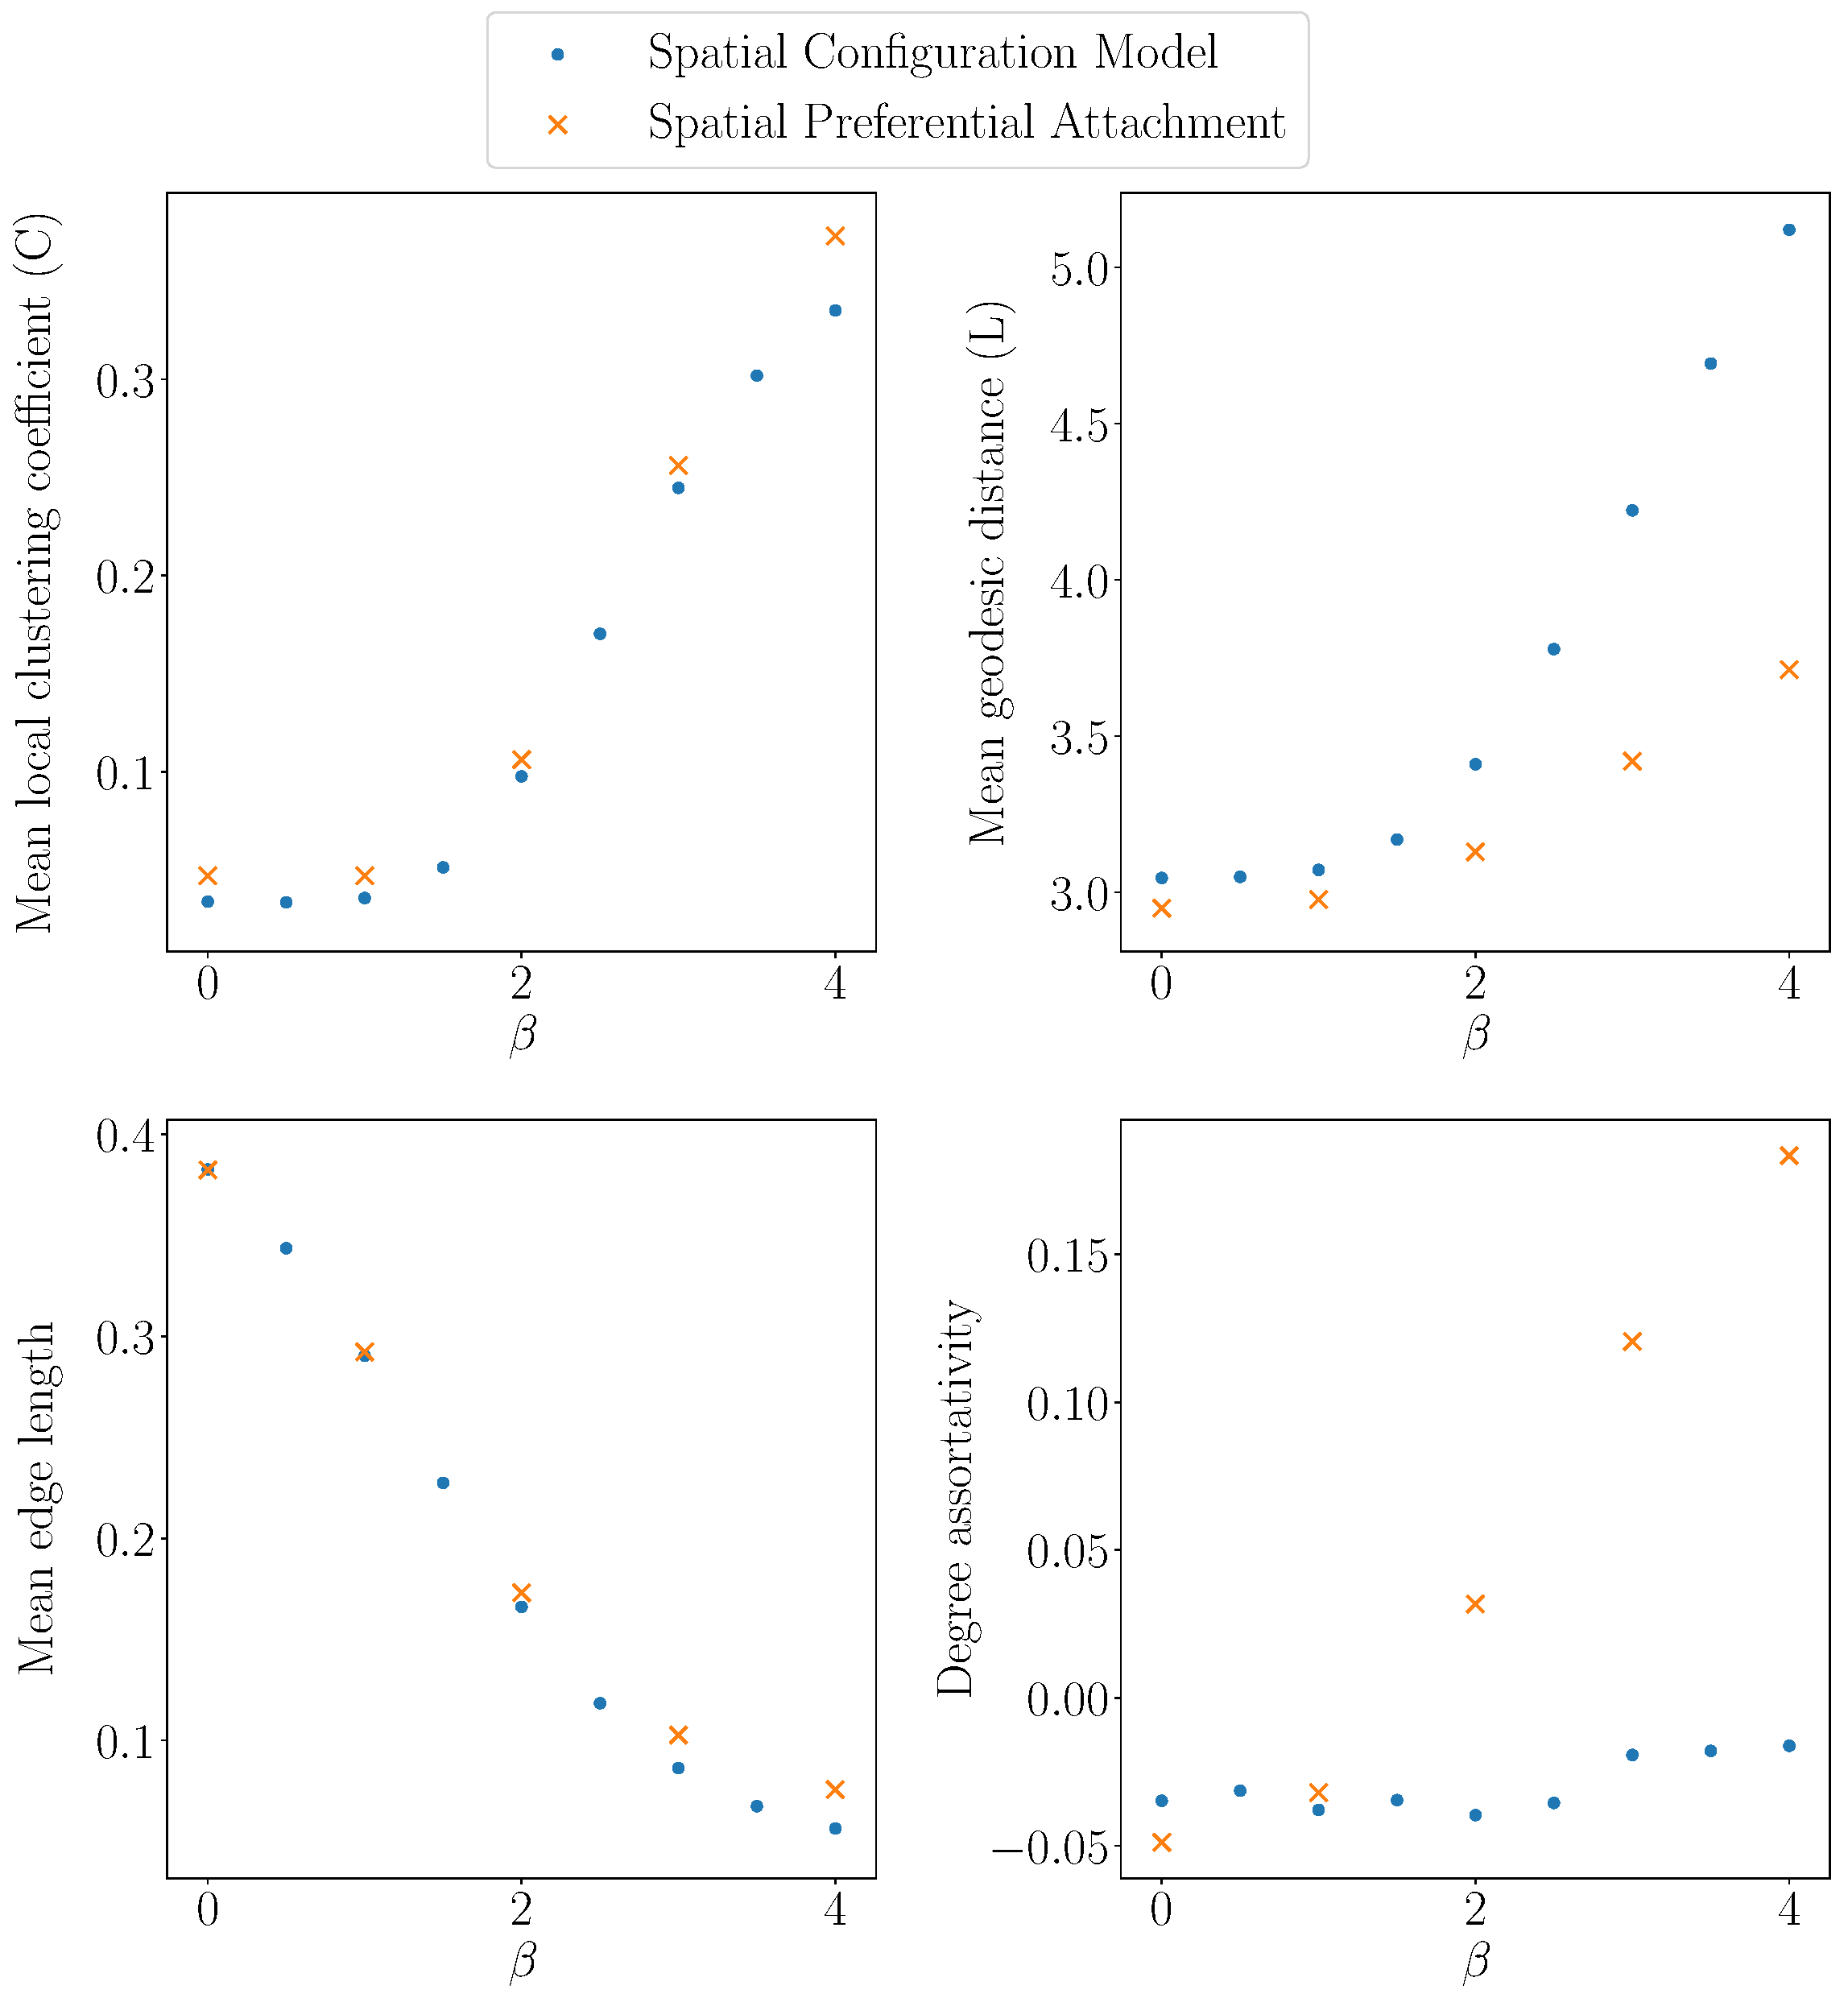
\includegraphics[width=1.0\linewidth]{spatial_preferential_comparison.pdf}
    \caption{Comparison of the characteristics of our spatial configuration model networks (blue circles) with characteristics of SPA networks (orange crosses) with $n = 1010$ nodes and $m = 5$ new edges for each node that we add. {\color{red}The spatial configuration networks are the same networks (configurations of BA models) used to plot Fig.~\ref{fig:spatial_configuration_metrics}, while the SPA networks are the same as were generated in Section \ref{sec:ba-model}.}
}
    \label{fig:spatial_preferential_comparison}
\end{figure}
    

In our spatial configuration model, we observe (as in the {\color{red}SPA and GF} models) that as we increase the spatial decay parameter $\beta$, the mean local clustering coefficient and mean geodesic distance increase, whereas the mean edge length decreases. The degree assortativity of networks from our spatial configuration model does not appear to have a clear correlation with $\beta$, unlike with the {\color{red}SPA and GF models.}

For comparison, we include an additional scatter plot of these characteristics for our spatial configuration model (for which we use degree sequences generated by BA networks), {\color{red} alongside scatter plots from our SPA network from Section \ref{sec:ba-model}. They both use a $10$-clique as the seed network, with the same total number of nodes ($n=1010$), and the same number of new edges per node that we add ($m=5$). }

%%%%%

\section{Spatial Strength Centrality Measure} \label{sec:spatial_strength}

Our explorations of spatial network models raise an interesting question: Can we quantify how strong the effects of the spatial embedding and choice of spatial decay function $h(r)$ are? We have observed that larger values of the spatial decay parameter $\beta$ lead to more prominent spatial effects on network topology. However, it is desirable to be more systematic about our analysis of spatial networks. For example, it is important to compare different choices of the function $h(r)$, different sizes and dimensions of the ambient space, and different distributions of nodes in space. Therefore, we define a centrality measure for spatial networks that we call \emph{spatial strength centrality}, and compare it across several synthetic and empirical spatial networks.

%%%%

\subsection{Definition and description of spatial strength centrality}


To develop a notion of centrality for spatial networks, we proceed as follows. {\color{red}Let $N(v_i)$ the neighborhood of $v_i$ (the set of nodes to which node $v_i$ is adjacent)}.
%{\bf andy: I ended up using $N(v)$ earlier, so changed up the wording here}
We then calculate the {\color{red}normalized} mean edge distance --- which we take to be Euclidean for concreteness, but one can also consider other metrics --- from node $v_i$ to each other node in its neighborhood. For a node $v_i$ with at least one incident edge, this distance is
\begin{align}
    L(v_i) = \frac{\sum_{v_j \in N(v_i)}d(v_i, v_j)}{k_i} \frac{1}{{\langle L \rangle}}\,,
\label{eq:v_edge_length}
\end{align}
where
\begin{align}
    \langle L \rangle = \frac{\sum_{(v_i, v_j) \in E}d(v_i, v_j)}{n \langle k \rangle}
\end{align}
and $d(i, j)$ is the Euclidean distance between nodes $v_i$ and $v_j$. The left fraction in $L(v_i)$ gives the mean edge length of $v_i$; we then normalize it by $\langle L \rangle$, the mean edge length in the network. We now calculate the mean neighbor degree of each node $v_i$ and normalize it by the mean degree in the network. That is,
\begin{equation}
    K(v_i) = \frac{\sum_{v_j \in N(v_i)} k_j}{k_i} \frac{1}{\langle k \rangle}\,.
\end{equation}
We then combine the above two quantities to calculate the spatial strength centrality
\begin{equation} \label{eq:spatial_strength}
    S(v_i) := \frac{1}{L(v_i)K(v_i)}
\end{equation}
of each node $v_i$ with at least one incident edge.

Our motivation in defining $S(v_i)$ is to capture a notion of whether nodes are adjacent to each other because they are spatially close or because they are adjacent to each other for a topological reason. Heuristically, we ``reward'' a node for being adjacent to spatially close nodes, and we ``penalize'' it for being adjacent to ``hubs'' (i.e., to nodes with large degree).

As an example, consider a network of flights between airports. Suppose that a small airport $v_i$ is adjacent only to a hub $v_j$, which is also far away from it geographically. Node $v_i$ has a small spatial strength $S(v_i)$ because its edge to $v_j$ does not arise from it being nearby, but instead because $v_j$ is a hub. This idea is captured by $S(v_i)$ because both $L(v_i)$ and $K(v_i)$ are large, as the one edge of $v_i$ is a long edge and its neighbor has large degree.
%is a hub with large degree).  {\bf map: previously, a hub automatically has large degree; if you are going to write this comment, you need to distinguish carefully from hubs that have large degree and hubs that do not; I believe "large degree" is what you actually mean (not actually any notion of being a hub)}
Therefore, from \eqref{eq:spatial_strength}, we see that $S(v_i)$ is small.

Conversely, consider a granular network \cite{papa2018}. In this network, nodes are adjacent if they are touching (or at least sufficiently close to be construed as touching). Moreover, because of physical constraints, the number of edges that are attached to a node is limited to be a small number.
Therefore, an arbitrary node $v_j$ in this network has short edges, so $L(v_j)$ is small. Additionally, every node in the neighborhood of $v_j$ has small degree, so $K(v_j)$ is small. {\color{red}Therefore, from \eqref{eq:spatial_strength}, we see that $S(v_j)$ is larger in this example than $S(v_i)$ from the previous airport example. }

%{\bf map: "larger" \emph{than what?} the other half of the comparison above is missing! Do you even mean to make an explicit comparison here?}


It can also be informative to calculate a network's mean spatial strength centrality
\begin{equation}
    \langle S \rangle = \frac{\sum_i S(v_i)}{n}\,.
\end{equation}
In the previous examples, for instance, we expect a granular network to have a larger value of $\langle S \rangle$ than the air-traffic network does, because the former's network topology has more stringent constraints from the system. 

%For simplicity, in the rest of this paper, we denote the mean spatial strength of a network as $S$ instead of $\langle S \rangle$.
%{\bf map: I am not so keen on this notational shorthand...}

There are several important considerations for calculating mean spatial strength:
\begin{enumerate}
    \item We have normalized all quantities, so we expect to be able to meaningfully compare the value of $\langle S \rangle$ for different types of networks, including ones with different size scales and spatial embeddings. However, $\langle S \rangle$ is unbounded (in particular, it is not confined to values between $0$ and $1$), so we need to be careful about interpreting its values and comparisons of these values.
    \item The mean spatial strength $\langle S \rangle$ is nonnegative.
    \item We normalized $K(v_i)$ by the mean degree $\langle k \rangle$, rather than by the largest degree $k_{\mathrm{max}}$ in a network, so it is not guaranteed to lie between $0$ and $1$.
    \item Our formulas for $L(v_i)$ and $S(v_i)$ are not well-defined for nodes that have no edges, so we take these quantities to be $0$ in these cases.
\end{enumerate}

%%%%

\subsection{Computation of spatial strength on network models}\label{sec:computed_ss}

As an initial test case, we consider the spatial strength centrality of the models that we defined earlier: the GF model, SPA model, and the spatial configuration model. We expect the mean spatial strength $\langle S \rangle$ to increase as we increase the spatial decay parameter $\beta$ (see Fig.~\ref{fig:spatial_model_strength}).


\begin{figure}
    \centering
    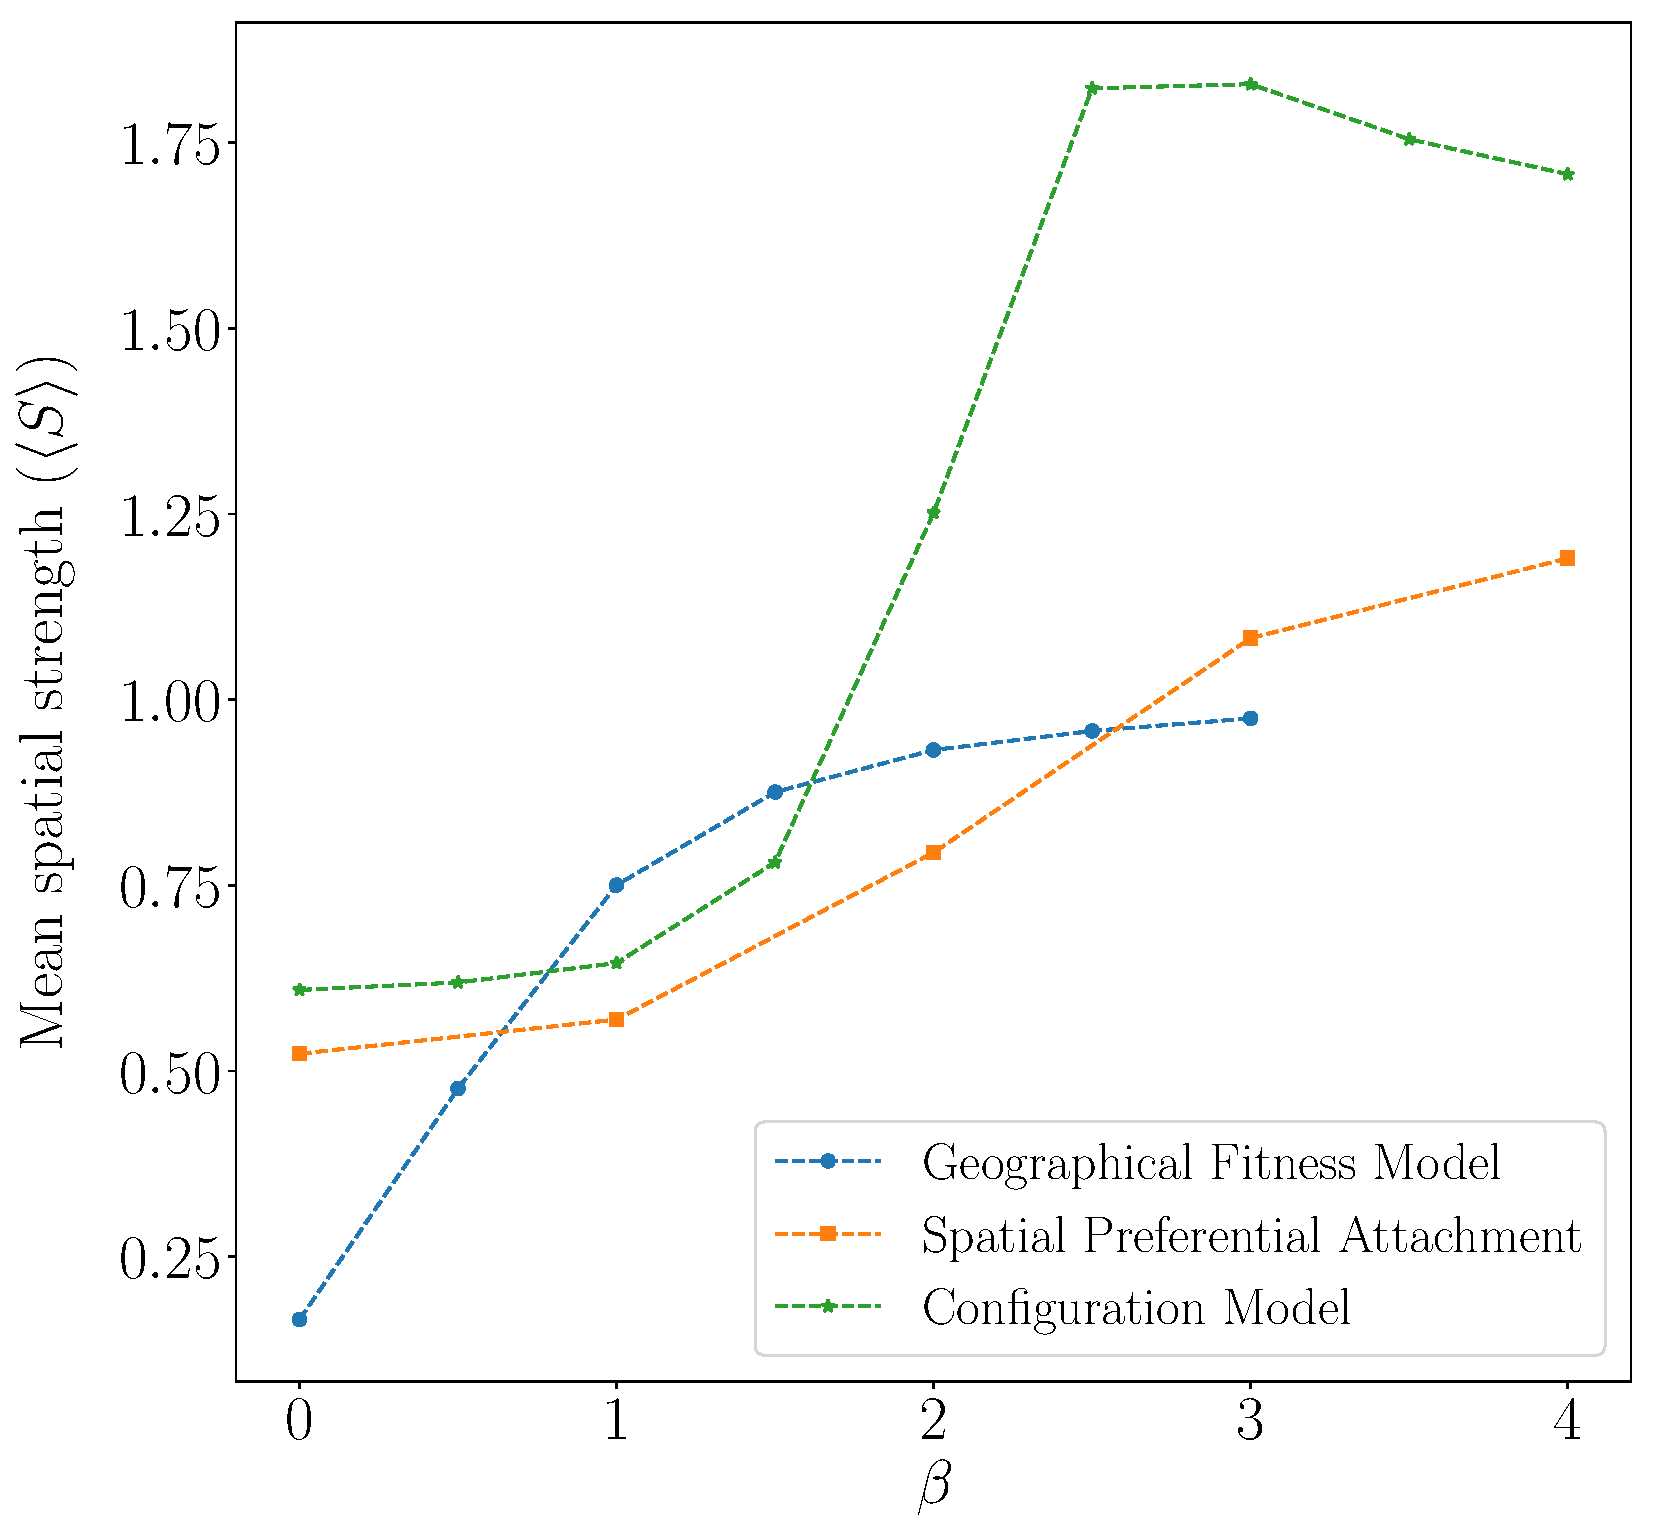
\includegraphics[width=1.0\linewidth]{spatial_model_spatial_strengths2.pdf}
    \caption{Mean spatial strength for our geographical fitness model, our SPA model, and the spatial configuration model for various values of the spatial decay parameter $\beta$. For a given value of $\beta$, each point represents a mean over $20$ realizations of the model. Our geographical-fitness-model networks have $n=500$ nodes, and our SPA and spatial-configuration-model networks have $n=1010$ nodes.
    }
    \label{fig:spatial_model_strength}
\end{figure}


Interestingly, although there is generally a positive correlation between $\beta$ and $\langle S \rangle$, it is not a linear relationship. The spatial configuration and SPA models yield S-shaped curves, and the GF model has an initially rapid increase of $\langle S \rangle$ with $\beta$ before tapering off.

Contrary to expectations (which were for $\langle S \rangle$ to tend to increase with $\beta$), for the spatial configuration model, the mean spatial strength reaches a peak at about $\beta = 3$.
 %(intuitively we expect mean spatial strength to be a non-decreasing function of $\beta$). 
 {\color{red}For progressively larger $\beta$, the mean edge length of a network decreases, in turn decreasing the mean spatial strength (since $L(v_i)$ increases as $\langle L \rangle$ decreases according to (\ref{eq:v_edge_length}), thus $S(v_i)$ decreases as $\langle L \rangle$ decreases). This sensitivity to mean edge length is a potential weakness in the centrality measure, and in Section \ref{sec:alternate_formations} we discuss potential ways to address this. }

%{\bf map: "later": let's turn this into an explicit pointer; in which Section do we do this?}




\begin{figure}
    \centering
    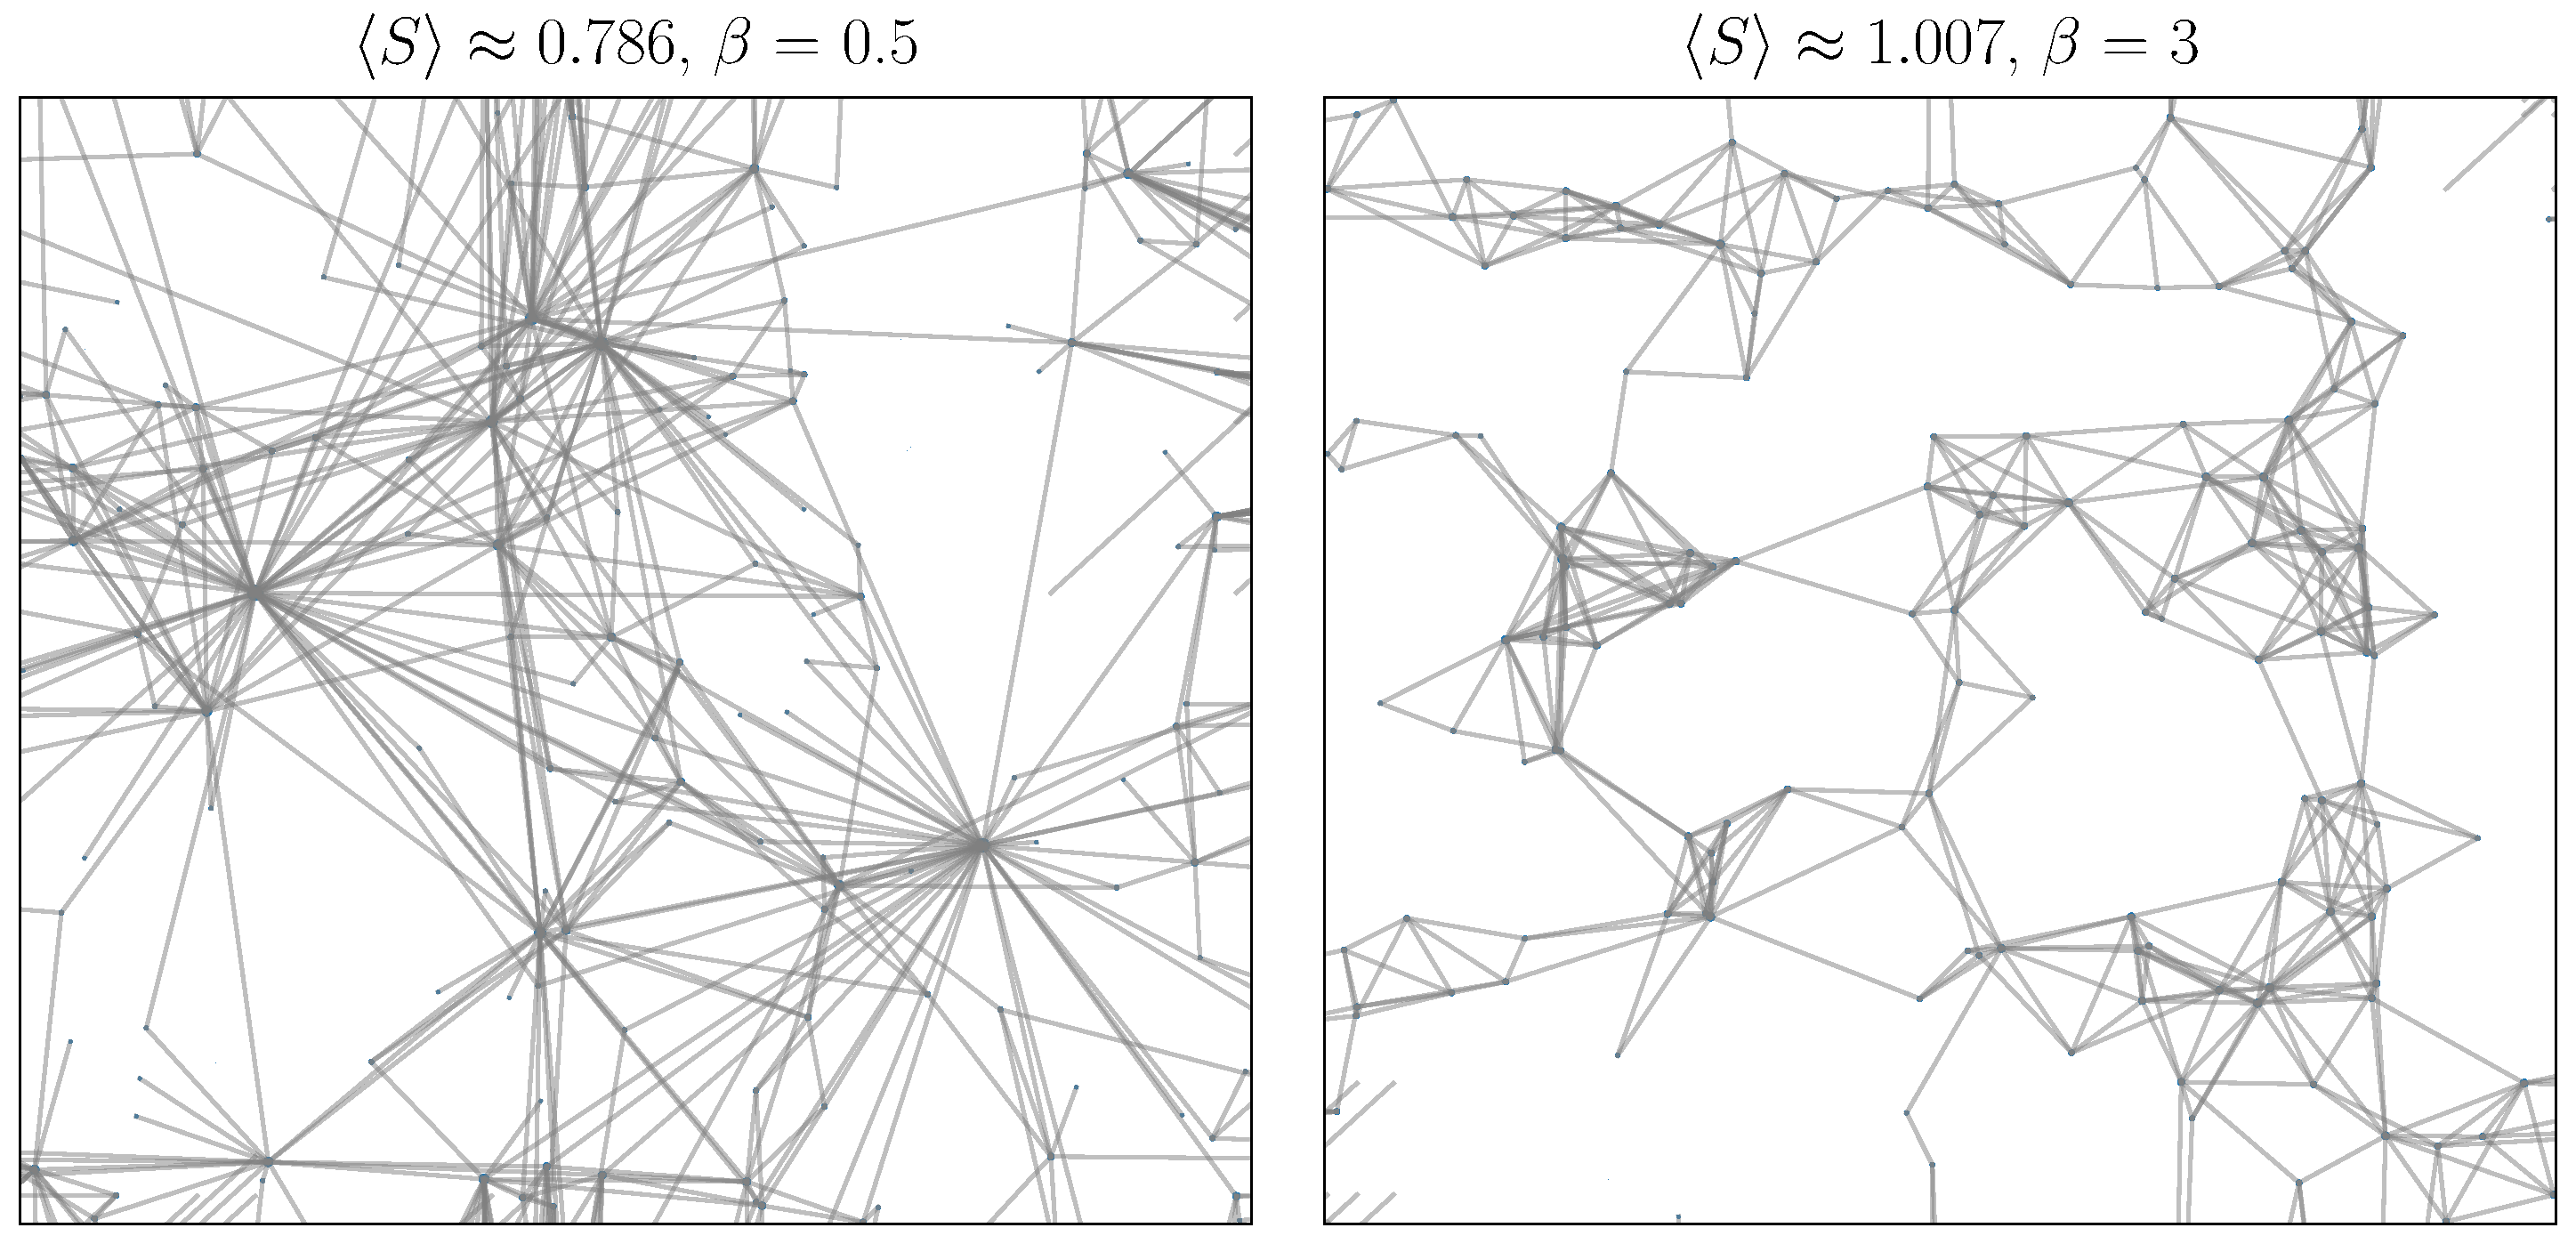
\includegraphics[width=1.0\linewidth]{geographic_example_no_highlight2horiz.pdf}
    \caption{Example networks from individual instantiations of the geographical fitness model with $n=150$ nodes, which we place in 2D according to their assigned coordinates. We show examples with (left) $\beta = 0.5$ and $\langle S \rangle \approx 0.786$ and (right) $\beta = 3$ and $\langle S \rangle \approx 1.007$. 
    }
    \label{fig:network_visualizations}
\end{figure}

%%%%%

\subsection{Examination of spatial strength on toy synthetic networks}

In Fig.~\ref{fig:network_visualizations}, we show individual instantiations of the GF model. To aid in developing intuition about the structure of networks that arise from this model, we also indicate their mean spatial strength centralities. To develop intuition about the centrality measure, we examine spatial strength centrality for several toy examples. We consider the following networks:
\begin{itemize}
\item{\textbf{Square lattice.} The lattice network has $x$ columns and $y$ rows, giving it a total of $n = xy$ nodes. We space these nodes evenly in $[0,1] \times [0,1]$, and each node is adjacent to the nodes that are immediately north, south, east, and west of it. See the left plot of Fig.~\ref{fig:toy_network_examples}. When $x=y$, the mean spatial strength tends towards $1$ as $n^2 \rightarrow \infty$.
}
\item{\textbf{Spatially-embedded Cayley tree.} This network has $b$ branches and $l$ layers. We start with one central node (layer $0$). Inductively, every node in layer $l$ is adjacent to $b$ nodes in layer $l+1$, whose nodes are equally spaced in a circle of radius $l+1$. See the center plot of Fig.~\ref{fig:toy_network_examples}. 
}
\item{\textbf{Hub-and-spoke example.} This example has three ``hub'' nodes that are each spaced relatively far away from its $10$ ``spoke'' nodes, which occur a circle around it. See the right plot of Fig.~\ref{fig:toy_network_examples}. This example demonstrates that a network with long-range connections can have a small mean spatial strength centrality. 
%This gives an intuition for the airline-flight network in Section \ref{data}.
}
\item{\textbf{Two-scale example.} Exploiting the definition of spatial strength centrality, we construct a network that consists of two pairs of nodes, where the nodes of each pair are adjacent to each (see Fig.~\ref{fig:breaking_example}). By making one edge short and the other arbitrarily large, the mean spatial strength centrality approaches infinity as the second edge becomes arbitrarily long. Therefore, we see that there exist networks with arbitrarily large values of mean spatial strength centrality. 
}
\end{itemize}



\begin{figure}
    \centering
    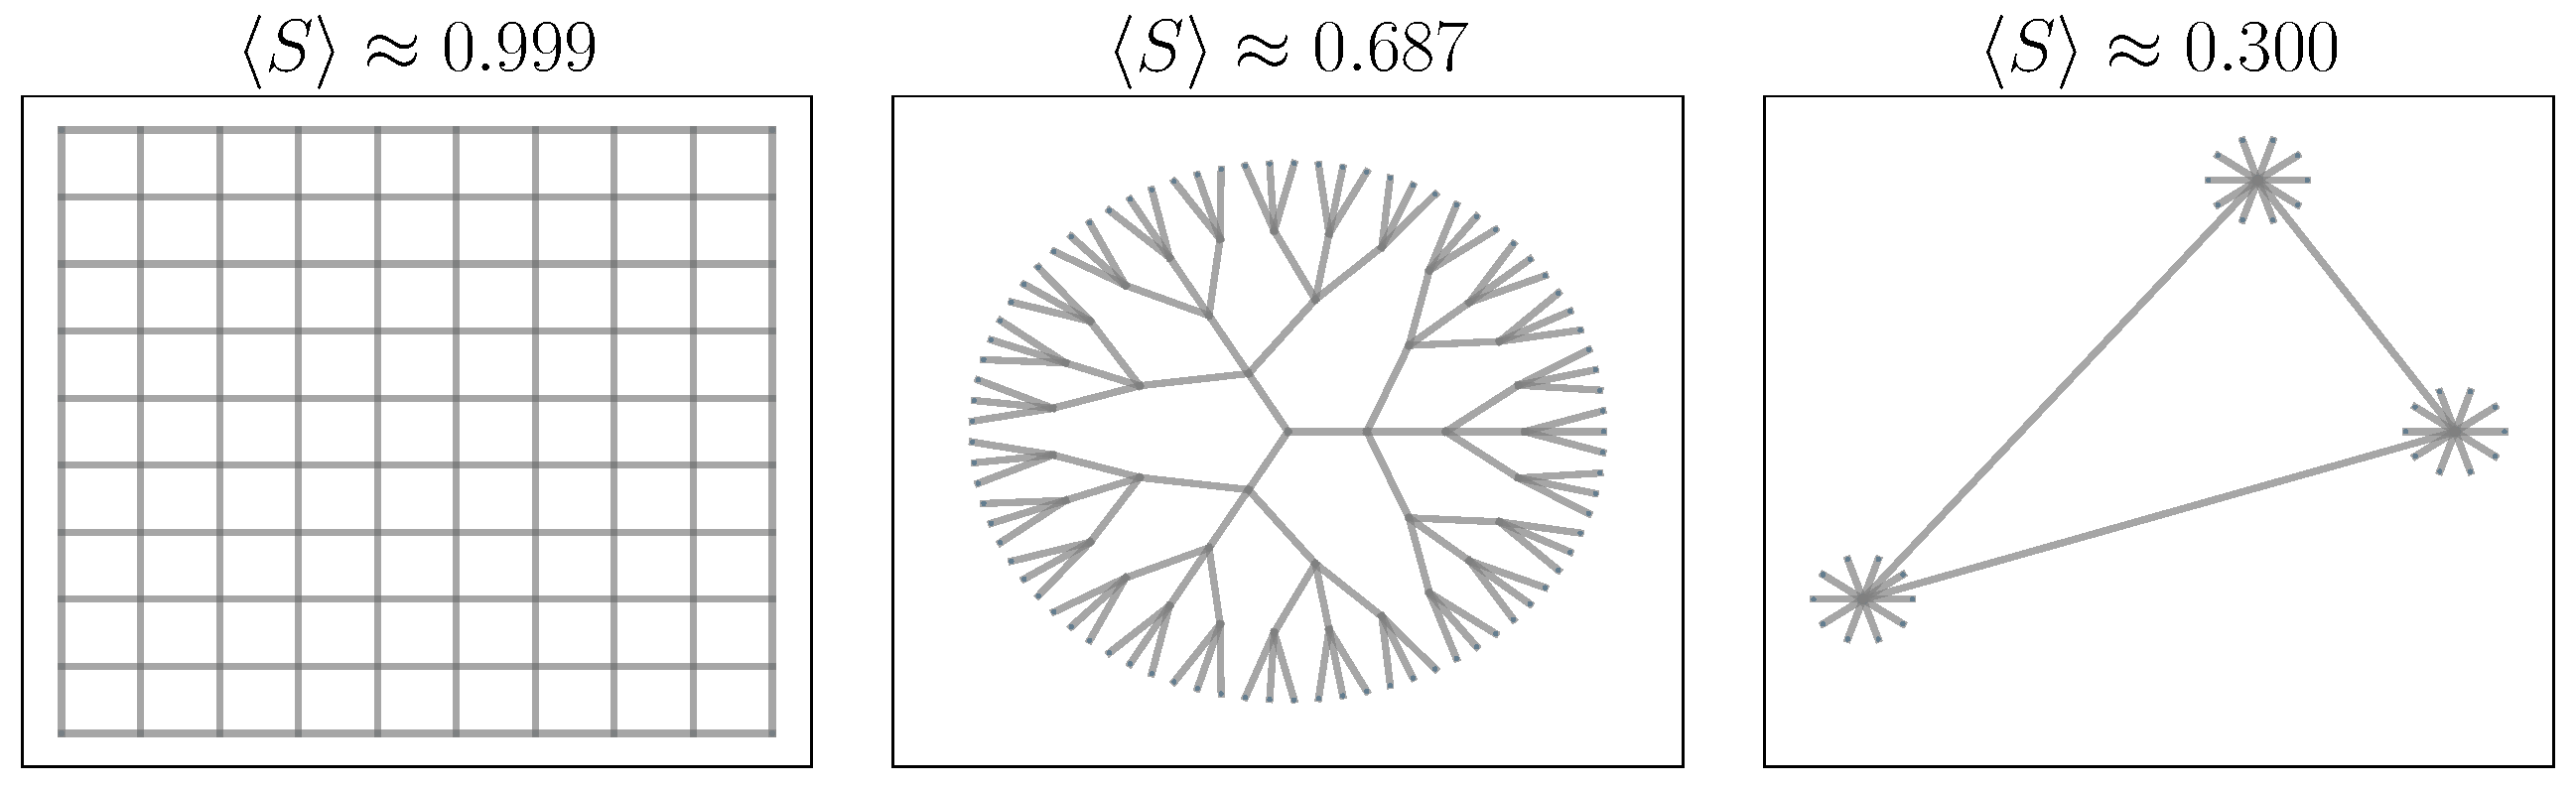
\includegraphics[width=1.0\linewidth]{toy_network_examples.pdf}
    \caption{Example networks with the indicated values for mean spatial strength. The depicted networks are (left) a lattice network, (center) a spatially-embedded Cayley tree, and (right) a hub-and-spoke example.
    }
    \label{fig:toy_network_examples}
\end{figure}




\begin{figure}
    \centering
    
\includegraphics[width=0.4\linewidth]{breaking_example_spatial_strength.pdf}
    \caption{This example of a two-scale network with two pairs of nodes illustrates that the mean spatial strength centrality $\langle S \rangle$ can be arbitrarily large.
    }
    \label{fig:breaking_example}
\end{figure}

%%%%

\subsection{Examination of spatial strength centrality on empirical and synthetic data sets}\label{data}

We now examine spatial strength centrality of several empirical networks, as well as on an RGG, {\color{red}which we defined in \ref{sec:fitness_model}.}
The data sets for fungal networks are from \cite{fungal_data} (with $270$ networks with between $68$ and $2742$ nodes and a mean 
%size 
of $819$ nodes), and the data sets for city road networks are from \cite{road_data} (with $101$ networks with between $42$ and $3871$ nodes and a mean 
%size 
of $874$ nodes). We show some example networks and their mean spatial strength centralities in Fig.~\ref{fig:data_network_examples}.

{\bf map: check the numbers of networks in the data sets; for example, shouldn't the road networks have 100 data sets, not 101? I thought it was 20 cities from each of 5 continents, so what is the 101st network?}

{\bf Andy: I double-checked and there seemed to be 21 networks in the Africa folder, is this incorrect?}

\begin{figure*}
    \centering
    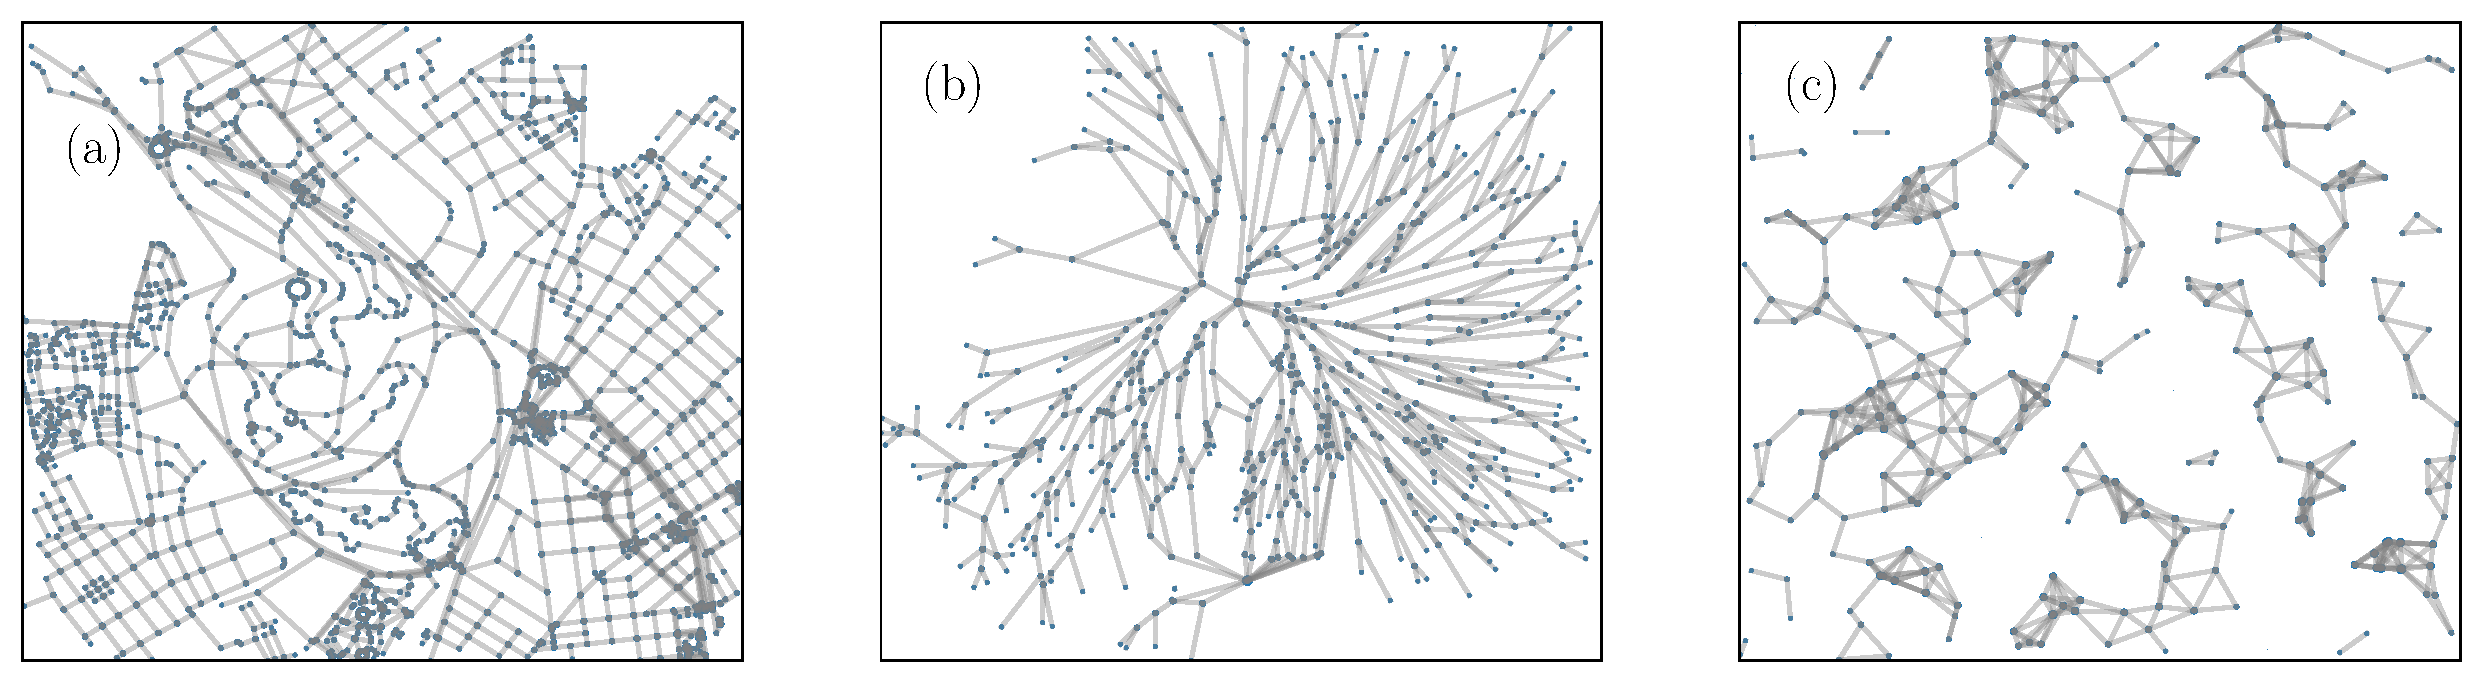
\includegraphics[width=1.0\linewidth]{data_network_examples.pdf}
    \caption{Example networks and mean spatial strength centralities empirical networks and a random geometric graph. We show (left) a road network from Tunis, Africa with $1731$ nodes; (center) a fungal network labeled ``Pv\textunderscore M\textunderscore I+4R\textunderscore U\textunderscore N\textunderscore 21d\textunderscore 4'' (see \cite{fungal_data}) with $641$ nodes; and (right) a random geometric graph with $n = 500$ nodes and distance parameter $r_c = 0.07$.
    }
    \label{fig:data_network_examples}
\end{figure*}


%It is worth noting that n
None of the model networks that we have explored thus far in the paper have yielded a mean spatial strength of greater than $2$.
 %(including the RGG model). 
 However, many of the networks in both the city road and fungal data sets have a mean spatial strength centrality that is larger than $2$. Therefore, there are structural features in spatial networks beyond the ones in the models in this paper.

%From surveying of some of the networks in the data sets that have the largest spatial strengths, we observe that they include areas of space in which nodes are very close together. 
{\color{red}We observed that in networks in the data sets with the greatest $\langle S \rangle$, there were areas of space in which nodes are very close together.}
For example, in a city road network (see the left side of Fig.~\ref{fig:data_network_examples}), multiple nodes (i.e., street intersections) can occur along curves in a road. Such nodes tend to have short edges between them and these networks, therefore, include edges at multiple spatial scales. As we saw in the example in Fig.~\ref{fig:breaking_example}, having both very long edges and very short edges can yield a large mean spatial strength centrality.



\begin{figure}
    \centering
    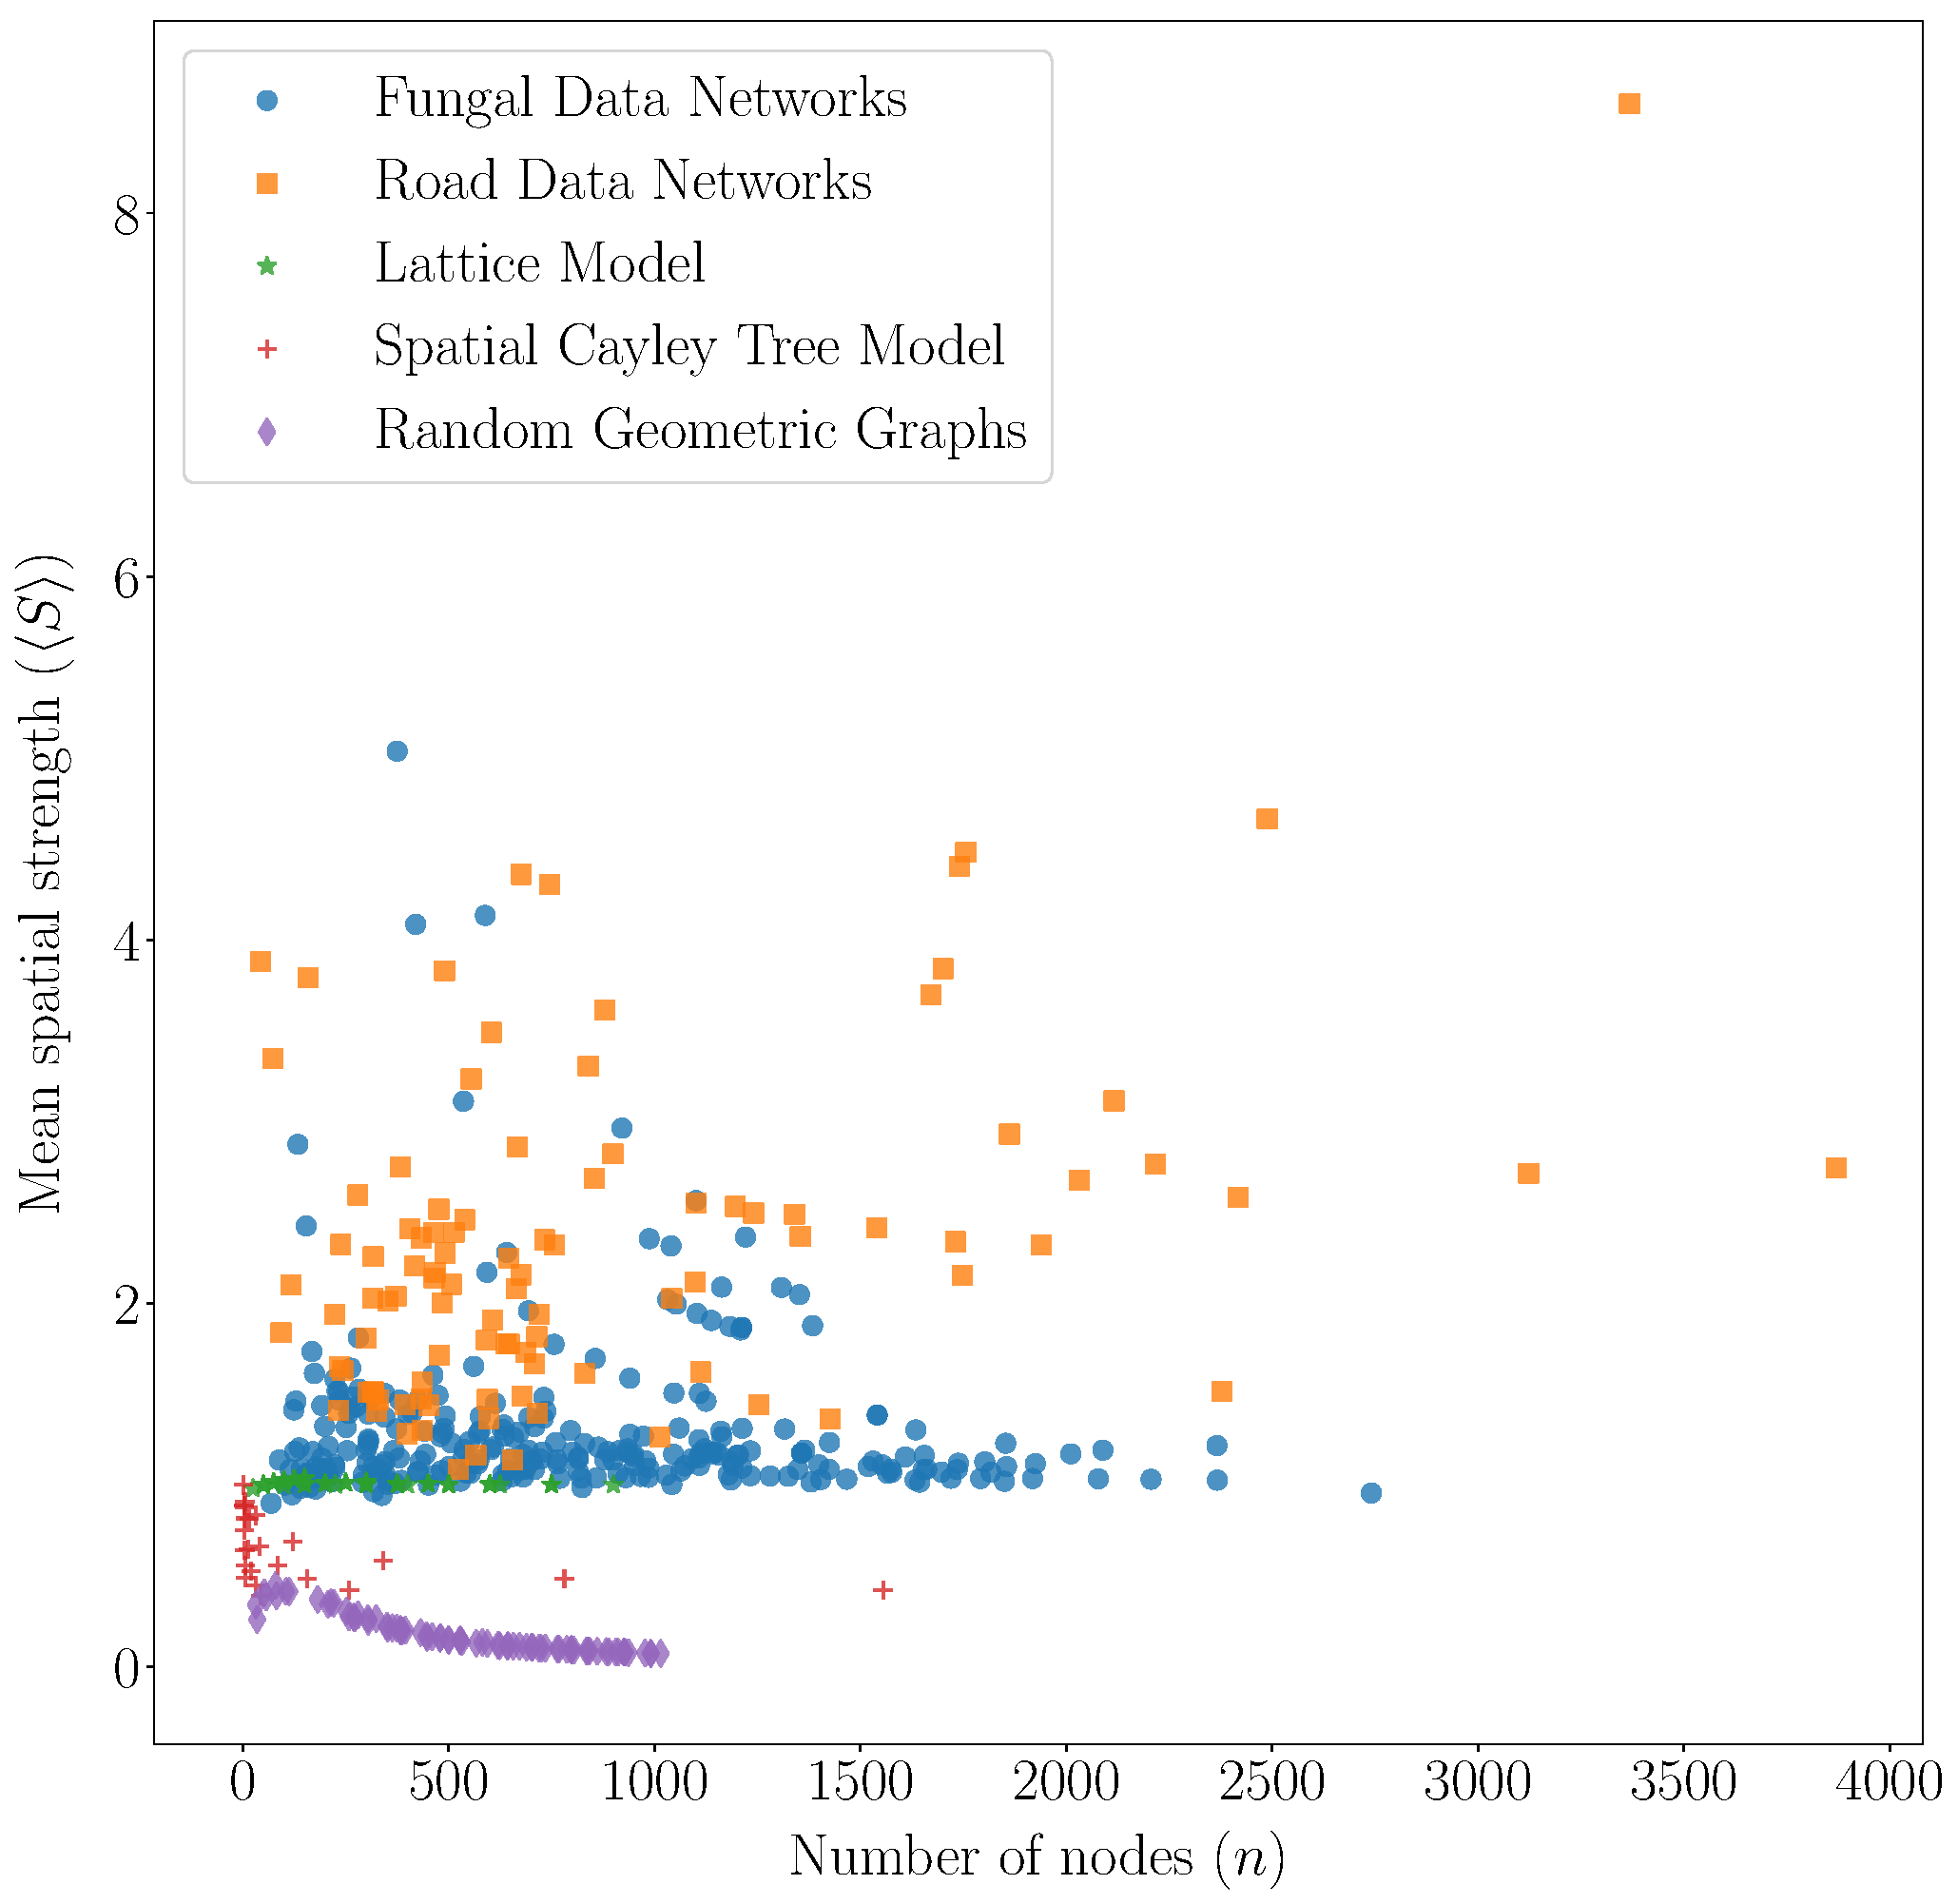
\includegraphics[width=1.0\linewidth]{spatial_scatter_1.pdf}
    \caption{Scatter plot of mean spatial strength versus the number of nodes in several synthetic and empirical networks. We use fungal network data from \cite{fungal_data}, road network data from \cite{road_data}, and RGGs with a distance parameter of $r_c = 0.07$. The spatial Cayley trees in this plot range from $1$ to $6$ branches, and their depths range from $1$ to $4$. The lattice networks have $5$, $10$, $15$, $20$, $25$, or $30$ rows and columns (and any combination of rows and columns of those sizes); on the plot, these form an almost horizontal line at a mean spatial strength centrality of about $1$.
    }
    \label{fig:spatial_distributions}
\end{figure}


In Fig.~\ref{fig:spatial_distributions}, we show a scatter plot of many of these networks and their mean spatial strength centralities.
%, for a visual guide of these simulations.

%%%%

\subsection{Alternate formulations of spatial strength centrality}\label{sec:alternate_formations}

As we saw in the computations of spatial strength centrality, it sometimes captures some aspects of how spatial embeddings influencing network topology, but it was not always successful at doing so (e.g., the fact that $\langle S \rangle$ is not an increasing function of $\beta$ for the spatial-configuration-model networks). To explore these issues further, the following considerations are worth examining:
%we suggest several possible modifications of spatial strength centrality:
\begin{itemize}
    \item{\textbf{Calculating spatial strength centralities for edges.} In (\ref{eq:spatial_strength}), we defined spatial strength centrality as a combination of mean neighbor degree and the mean edge length of a node. One might instead consider the ``spatial strength'' of edges instead of nodes. {\color{red}For example, for an edge $(i, j)$ one could sum the degrees of $v_i$ and $v_j$, and divide by the length of the edge $r_{i,j}$. }}
%Another way to formulate a spatial strength centrality is to calculate a ``spatial strength'' of each edge, such as by multiplying the inverse of edge length by the neighbor degrees of nodes that are incident to the edge. {\bf map: what exactly do you mean by "neighbor degree"? specifically, what is the precise difference between "neighbor degree" and "degree"? I would interpret those two objects to be different, so I don't know the definition of the concept you have in mind}}
    \item{\textbf{Normalization of mean edge length.} We noted (see Section \ref{sec:computed_ss}) that $\langle S \rangle$ is sensitive to mean edge length. This is because $L(v)$ increases and $S(v)$ decreases as $\langle L \rangle$ decreases. 
     %{\bf map: "(as for the configuration model data, $\langle S \rangle$ decreased as $\beta$ increased beyond $3$, which was counter to our expectations).": I'm not following this statement; also, I don't think we ever stated this before (though it's in the picture), and I definitely don't remember this being mentioned in the context of 'sensitivity'; I am lost} 
     {\color{red}It may instead be useful to normalize $L(v)$ by the maximum pairwise edge length in a network, rather than by the mean edge length. 
     
     The point of normalizing $L(v)$ by mean edge length is to be able to compare networks of different sizes. An alternate way to do this would be to normalize $L(v)$ by the geographic diameter of the network, possibly as measured by the maximum pairwise distance between nodes of the network.}}
    \item{\textbf{Comparison of a spatial network to null models.} The goal of calculations of spatial strength centrality is to determine {\color{red}how a network's spatial embedding affects its topology}. To that end, instead of a centrality measure, it may be desirable to compare a given network to a spatial null model to determine how the spatial embedding affects the adjacency matrix (i.e., topology) of the network. For such purposes, the spatial configuration model may be useful as a null model.}
\end{itemize}

%{\bf map: item (3) is not a modification, so I changed the phrasing above that states what is in the bullets}

%%%%

\section{Conclusions and Discussion} \label{sec:discussion}

We have developed and examined a straightforward method for generalizing generative models of networks to incorporate spatial information by using a deterrence function $h(r)$ that decays with the distance $r$ between nodes to adjust the probability that an edge occurs between a pair of nodes. For concreteness, we used a Euclidean distance and the power-law decay rate $h(r) = r^{-\beta}$, but our formulation allows one to make diverse choices of both metric and decay function. 
%The reader may be interested in \cite{geometric_preferential_attachment, SPA4} for examples of networks embedded in non-Euclidean space.


One illustration of how to augment existing network models, rather than define new spatial network models from scratch, is with our formulation of a spatial configuration model. We also extended a GF model with $h(r)$, and examined a SPA model that used this deterrence function. 
%{\bf map: check the accuracy of the sentence above, especially in light of comments I wrote earlier}
We examined the properties of these models and compared them to random geometric graphs and empirical spatial networks from two disparate applications. To examine the structure of spatial networks more deeply --- and, in particular, to try to separate the effects of spatial embeddings and other influences on network architecture, we defined a spatial strength centrality, which allowed us to estimate how strongly the effects of a network's ambient space (in which its nodes are embedded) affects observed network topology. We examined spatial strength centrality on several toy networks and 
%then 
compared it on a diverse set of synthetic and empirical spatial networks.

Spatial networks have diverse uses in the modeling of networks from empirical data, and the models that we have examined in this paper should help in such efforts. We anticipate that further exploration of spatial null models (e.g., using our spatial configuration model and generalizations of it) will be particularly insightful, as they provide baselines for comparisons with empirical data. To explore the diverse effects of spatial embeddings (and other effects of space) on network topology, it is also important to further analyze deterrence functions $h(r)$ and a variety of notions of spatial strength centrality.



%%%%%

\section*{Acknowledgements}

{\color{red}We thank Heather Z. Brooks (University of California, Los Angeles) for helpful discussions.}

%{\bf map: is there anybody to thank? [I am a coauthor, so I commented out the thanking of me; are there any specific individuals (you wrote "other staff"), whether professors or postdocs or students, who we should thank by name?]}
%{\bf andy: I did talk with Professor Brooks about the project once or twice, but besides that no one else I believe. Is it okay to have an Acknowledgements section this short?}
%The authors thank Mason A. Porter and other staff at the University of California, Los Angeles math department, for guidance and advice in writing this paper.

%%%%

\bibliography{references2}

%%%%

\end{document}

%
% ****** End of file apssamp.tex ******